%%%%%%%%%%%%%%%%%%%%%%%%%%%%%%%%%%%%%%%%%%%%%%%%%%%%%%%%%%%%%%%%%%%%%%%%%%%%%%%%
%2345678901234567890123456789012345678901234567890123456789012345678901234567890
%        1         2         3         4         5         6         7         8

%\documentclass[preprint,5p]{elsarticle}
\documentclass[preprint,3p,times]{elsarticle}

\usepackage[utf8x]{inputenc}
\usepackage[T1]{fontenc}

\usepackage[english]{babel}
\usepackage{graphicx, subfigure}
\usepackage[usenames,dvipsnames]{xcolor}
\usepackage{tikz}
\usetikzlibrary{positioning}

\usepackage{amsmath} % \text

\usepackage{paralist}

\usepackage[draft,nomargin, marginclue, footnote]{fixme}

\usepackage{hyperref}

\newcommand{\concept}[1]{{\small \texttt{#1}}}
\newcommand{\stmt}[1]{{\footnotesize\tt$\langle$#1\relax$\rangle$}}

\usepackage{xspace}
\newcommand{\ie}{i.e.\xspace}
\newcommand{\cf}{{\textit{cf\ }}}
\newcommand{\eg}{e.g.\xspace}
\newcommand{\etal}{et al.\xspace}

\newcommand{\action}[3]{#1\\\textsf{\scriptsize #2,}\\\textsf{\scriptsize #3}}

\graphicspath{{figs/}}
\DeclareGraphicsExtensions{.pdf,.jpg,.png}

\begin{document}
\begin{frontmatter}

\title{\LARGE \bf
Artificial Cognition for Social Human-Robot Interaction:\\ An Implementation
}

\author{Séverin Lemaignan$^{1,2}$, Mathieu Warnier$^1$, E. Akin Sisbot$^1$,
    Aurélie Clodic$^1$, Rachid Alami$^1$}

\address{
$^1$LAAS-CNRS, Univ. de Toulouse, CNRS\\
7 avenue du Colonel Roche, F-31400 Toulouse, France\\
{\tt firstname.surname@laas.fr}
}

\address{
$^2$Centre for Robotics and Neural Systems\\
Plymouth University, Plymouth, United Kingdom\\
{\tt firstname.surname@plymouth.ac.uk}
}



%%%%%%%%%%%%%%%%%%%%%%%%%%%%%%%%%%%%%%%%%%%%%%%%%%%%%%%%%%%%%%%%%%%%%%%%%%%%%%%%
\begin{abstract}

Human-Robot Interaction challenges Artificial Intelligence in many regards:
dynamic, partially unknown environments that were not originally designed for
robots; a broad variety of situations with rich semantics to understand and
interpret; physical interactions with humans that requires fine, low-latency yet
socially acceptable control strategies; natural and multi-modal communication
which mandates common-sense knowledge and the representation of possibly
divergent mental models. This article is an attempt to characterize these challenges
and to exhibit a set of key decisional issues that need to be addressed for a
cognitive robot to successfully share space and tasks with a human.

We identify the needed individual and collaborative cognitive
skills: geometric reasoning and situation assessment based on perspective-taking
and affordance analysis; acquisition and representation of knowledge models for
multiple agents (humans and robots, with their specificities); natural multi-modal dialogue;
human-aware task planning; human-robot joint task achievement. The article
discusses each of these abilities, presents a working implementation, and shows
how they combine in a coherent and original deliberative architecture for
human-robot interaction. Supported by experimental results, we eventually show
how explicit knowledge management, both symbolic and geometric, proves to be
instrumental to richer and more natural human-robot interactions by pushing for
pervasive, human-level semantics within the robot's deliberative system.

\end{abstract}

\begin{keyword}
    human-robot interaction \sep cognitive robotics \sep perspective taking \sep knowledge representation and reasoning
\end{keyword}

\end{frontmatter}

%%%%%%%%%%%%%%%%%%%%%%%%%%%%%%%%%%%%%%%%%%%%%%%%%%%%%%%%%%%%%%%%%%%%%%%%%%%%%%%%

\section{The Challenge of Human-Robot Interaction}

\subsection{The Human-Robot Interaction Context}

Human-Robot Interaction (HRI) represents a challenge for Artificial Intelligence
(AI). It lays at the crossroad of many subdomains of AI and in effect, it calls
for their integration: modelling humans and human cognition; acquiring,
representing, manipulating in a tractable way abstract knowledge at the human
level; reasoning on this knowledge to make decisions; eventually instantiating
those decisions into physical actions both legible to and in coordination with
humans.  Many AI techniques are mandated, from visual processing to symbolic
reasoning, from task planning to \emph{theory of mind} building, from reactive
control to action recognition and learning.

We do not claim to address here the issue as a whole. This article attempts
however to organise it into a coherent challenge for Artificial Intelligence,
and to explain and illustrate some of the paths that we have investigated on our
robots, that result in a set of deliberative, knowledge-oriented, software
components designed for human-robot interaction.

%The proposed scheme is specially designed for  interaction, and more particularly cooperative task achievement by one robot and one or several humans - called here the robot human partners. It is applicable to domains such as assistant or service robots in domestic and public places as well as to teammate robots in the factory of the future.

We focus on a specific class of interactions: human-robot collaborative task
achievement~\cite{alami2013human} 
supported by multi-modal and situated communication. Figure~\ref{fig:hri-dec}
illustrates this context: the human and the robot share a common space and exchange
information through multiple modalities (we specifically consider verbal
communication, deictic gestures and social gaze), and the robot is expected to achieve
interactive object manipulation, fetch and carry tasks and other similar
chores by taking into account, at every stage, the intentions, beliefs,
perspectives, skills of its human partner.  Namely, the robot must be able to
recognise, understand and participate in communication situations, both explicit
(\eg the human addresses verbally the robot) and implicit (\eg the human points
to an object); the robot must be able to take part in joint actions, both
pro-actively (by planning and proposing resulting plans to the human) and
reactively; the robot must be able to move and act in a safe, efficient and
legible way, taking into account social rules like proxemics.

\begin{figure}[htb]
\centering
\begin{tikzpicture}
    \node at (0,0) {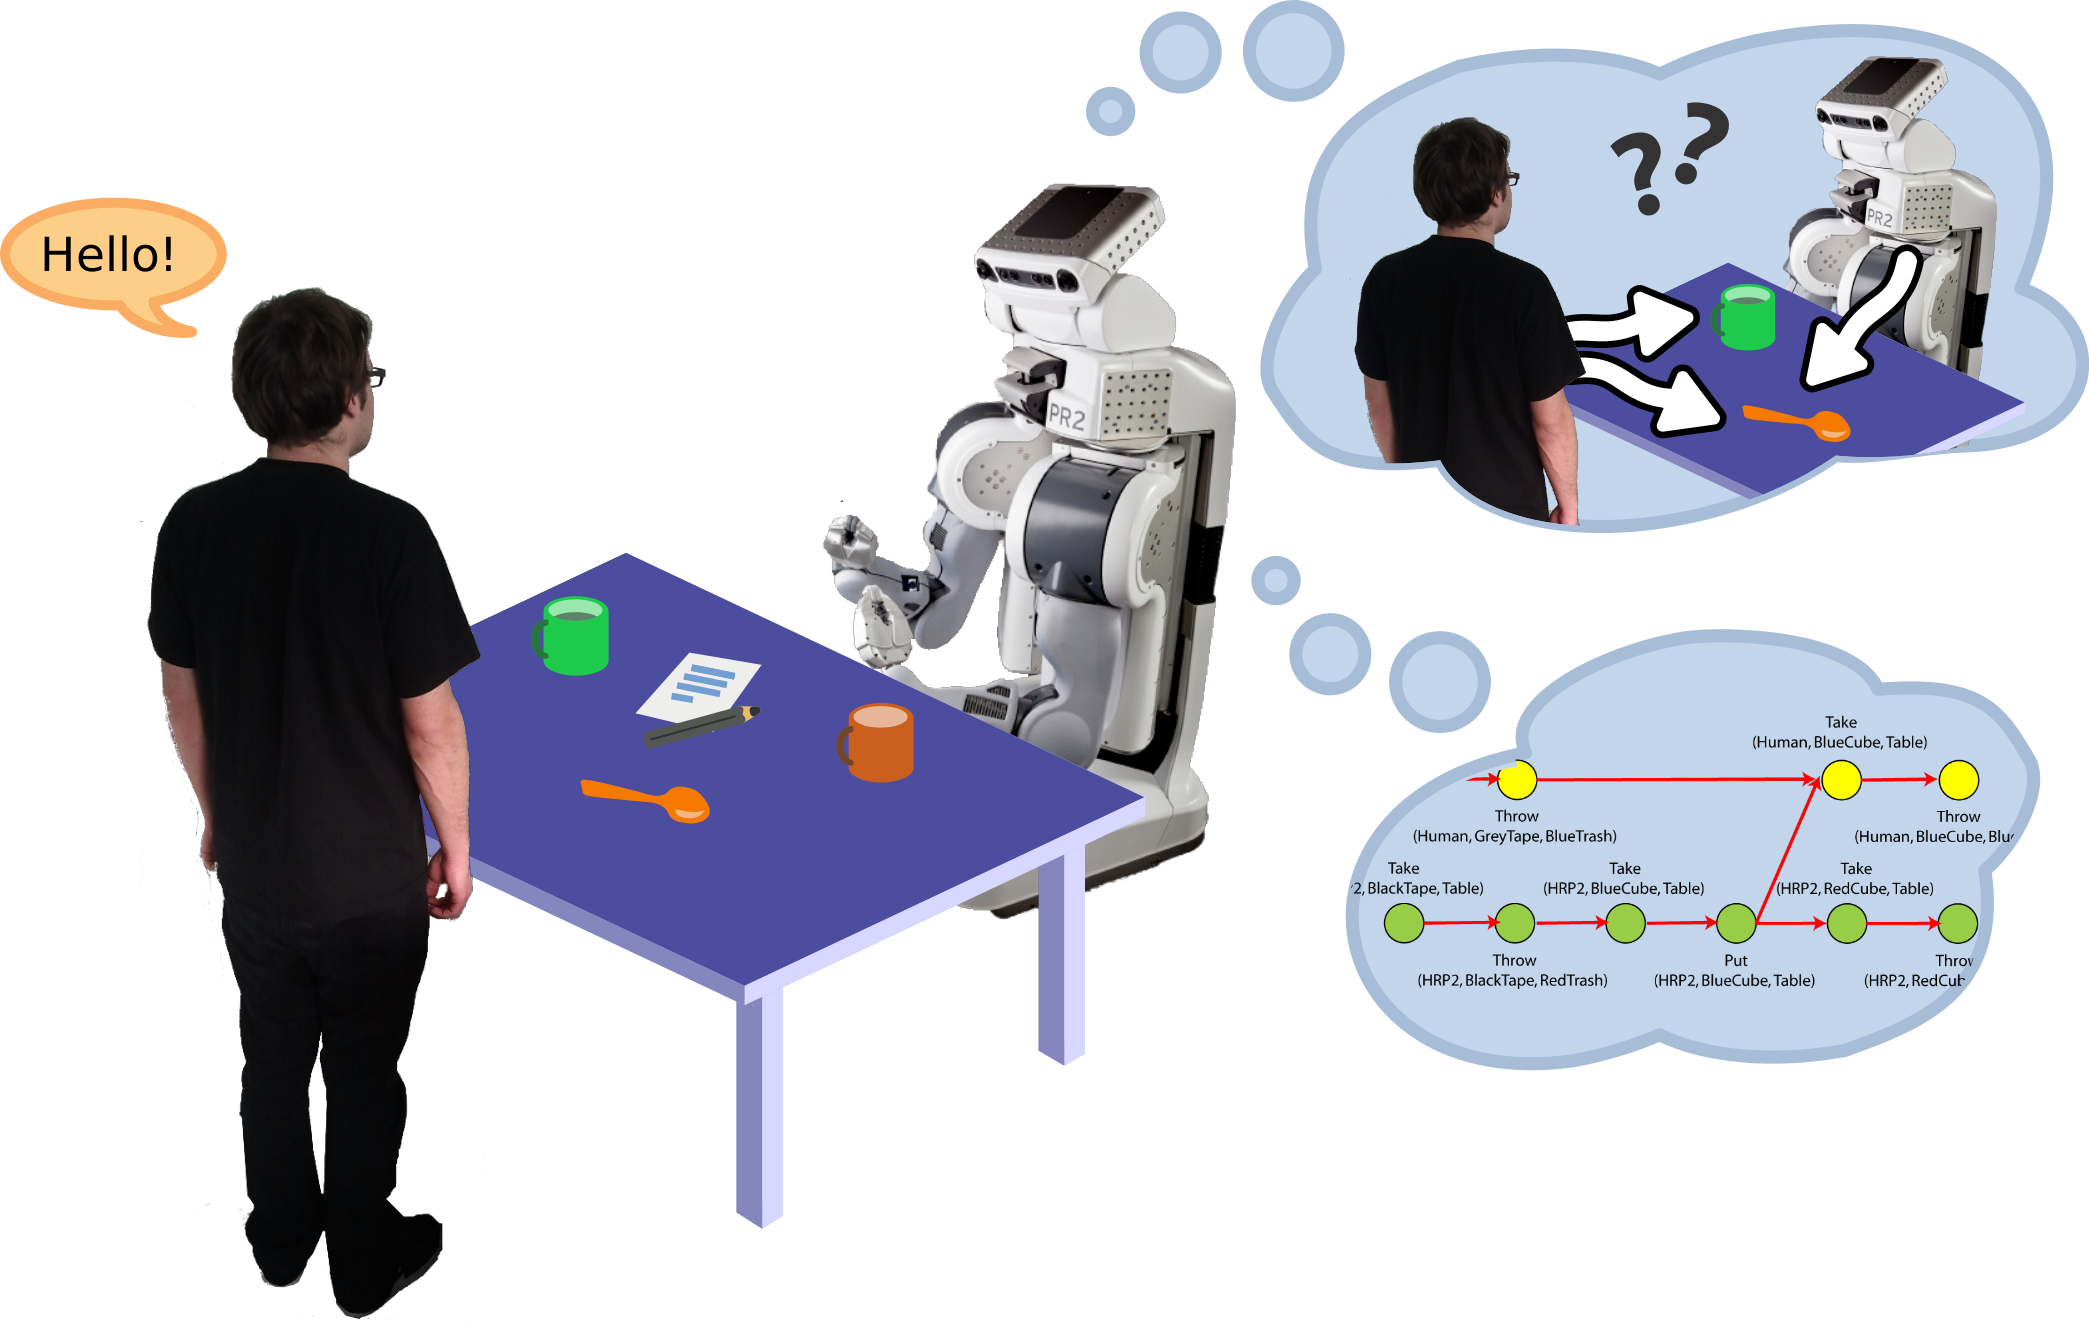
\includegraphics[width=0.6\textwidth]{grounding_robot.png}};
    \node[circle, draw] at (-3.5,2.5) {A};
    \node[circle, draw] at (5.5,2) {D};
    \node[circle, draw] at (5.2,-1) {C};
    \node[circle, draw] at (-1,2) {B};
\end{tikzpicture}

\caption{The robot reasons and acts in domestic interaction scenarios.  The
    sources of information are multi-modal dialogue {\it (A)} and
    perspective-aware monitoring of the environment and human activity {\it
    (B)}. The robot must adapt on-line its behaviours by merging computed plans
    {\it (C)} with reactive control. The robot explicitly reasons on the fact
    that it is (or not) observed by the human. Reasoning and planning take place
    at symbolic as well as geometric level and take into account agents beliefs,
    perspectives and capabilities {\it (D)} as estimated by the robot.}

\label{fig:hri-dec}
\end{figure}

These three challenges, \emph{communication}, \emph{joint action},
\emph{human-aware execution}, structure the research in human-robot
interaction. They can be understood in terms of cognitive skills that they
mandate. \emph{Joint action}, for instance, builds from:

\begin {itemize}
    \item a joint \emph{goal}, which has been previously established and agreed
        upon (typically through dialogue),
    
    \item a physical environment, estimated through the robot's exteroceptive
        sensing capabilities, and complemented by inferences drawn from previous
        observations,
    
    \item a belief state that includes {\it a priori} common-sense knowledge and
        mental models of each of the agents involved (the robot and its human partners).

\end {itemize}

The robot controller (with the help of a task planner) decides what action to
execute next, and who should perform it, from the robot or the human (or both in
case of a joint action). It finally controls and monitors its execution. The
operation continues until the goal is achieved, is declared unachievable or is
abandoned by the human~\cite{Klein2004}.

\begin{inparaenum}

This translates into several decisional, planning, representation skills that
need to be available to the robot~\cite{alami2011robot}. It must be able \item
to represent and manipulate symbolic belief states, \item to acquire and keep
them up-to-date with respect to the state of the world and the task at hand,
\item to build and iteratively refine shared (human-robot) plans, \item to
instantiate and execute the actions it has to perform, and conversely, to
monitor those achieved by its human partner.

\end{inparaenum}

Besides, such abilities should be designed and implemented in a task-independent
manner, and should provide sufficient levels of parametrization, so that they adapt to
various environments, different tasks and variable levels of engagement of the
robot, ranging from teammate behaviour to assistant or pro-active helper.

These are the challenges that we will discuss in this article.

\subsection{Contribution and Article Overview}

The main contributions concern the architecture of the decisional layer of a robot designed to share 
the space and the task with humans and to act and interact in a way that facilitates human action and decision.

We present a model of cognitive integration for service robots that:

\begin{itemize}

    \item achieves advanced grounding in complex real environments involving one or
        several humans and a robot;

    \item supports a distributed computation of symbolic knowledge for
        situated dialogue, thanks to the combination of perspective taking,
        affordances computation and logical inference;

    \item provides generic mechanisms for the robot to reason about the mental state
        of its human partners;

    \item reuses the same set of affordances and inferences, together with
        explicit contextual reasoning on humans and robot abilities, to generate
        human-robot shared plans;

    \item exposes a principled approach to integrate a set of complex cognitive
        components in an explicit, semantics-oriented and loosely-coupled
        fashion.

\end{itemize}

Importantly, this architecture is fully implemented and we demonstrate it on
several robotic platforms and in several actual interaction scenarios. It also proved
to be an effective framework for novel contributions about human-robot joint
action~\cite{fiore2016planning,devin2016implemented,milliez2016using}, as well
as for multi-disciplinary studies~\cite{dautenhahn2006may,koay2007exploratory,Ros2010b,dehais2011physiological,ferreira2015users,GharbiROMAN2015}.

\vspace{0.5cm}
The remaining of the article discusses the robotic architecture that we have
built to address social and autonomous human-robot interaction, and how it
relates to other approaches. We organise this discussion in four sections.

The next section introduces the architecture as a whole, as well as the
knowledge model that we have developed for our robots. Then,
Section~\ref{sec:impl} provides further details on each of the main components of the architecture.
Section~\ref{sec:expe} presents two studies that illustrate in a practical way
what can be currently achieved with our robots.  The
Sections~\ref{sect|discussion} and~\ref{sect|conclusion} finally summarize our
main contributions and discuss the key challenges that human-robot interaction
brings to Artificial Intelligence.



\section{Deliberative Architecture and Knowledge Model}


\begin{figure*}[ht]
\centering

\resizebox{\textwidth}{!}{%

\tikzset{subpart/.style={draw, font=\scriptsize, fill opacity=0.5, text opacity=1, fill=white!50}}

\begin{tikzpicture}[
    >=latex,
    every edge/.style={draw, very thick},
    skill/.style={draw, rounded corners, align=center, inner sep=5pt, fill=black!20},
    label/.style={midway, align=center, font=\scriptsize, fill=white}]

  %%% ORO
    \node at (0,0)[skill, ultra thick, fill=LimeGreen!50] (oro) {{\sc Oro} -- Symbolic facts \\ and beliefs management};
  
  %%% HATP
  \node at (-6, 2)[skill, fill=PineGreen!50] (hatp) {HATP -- Human-aware \\ symbolic task planning};
  
  %%% DIALOGS
  \node at (-6, -2) [skill, fill=BrickRed!50] (dialogs) {{\sc Dialogs} --
      Natural\\ language processing};

  %%% SPARK
  \node at (4,-3)[skill, fill=Purple!50] (spark) {%
      \begin{tikzpicture}
          \node at (0,0) (geom) {{\sc Spark} -- Geometric \& temporal situation assessment};
        \node [subpart, below=0.2 of geom.south west, anchor=north west] (world-update) {Sensors fusion};
        \node [subpart, right=0.2 of world-update] (geom-model) {Geometric model of the environment};
        \node [subpart, right=0.2 of geom-model] (fact-prod) {Symbolic facts production};
      \end{tikzpicture}
    };

  %%% MHP
    \node at (9,0)[skill, fill=BurntOrange!50] (mhp) {{\sc mhp} -- Human-aware \\ motion and manipulation \\ planning};

  %%% SHARY
  \node at (4,4)[skill, fill=RoyalBlue!50] (shary) {%
      \begin{tikzpicture}
          \node at (0,0) (exec) {{\sc Shary | pyRobots} -- Execution controllers};
        \node [subpart, below=0.2 of exec.south west, anchor=north west] (plans) {Goal \& Plans \\ management};
        \node [subpart, right=0.2 of plans] (sit-asses) {Situation assessment \\ and context management};
        \node [subpart, right=0.2 of sit-asses] {Action instantiation, \\ execution and monitoring};
      \end{tikzpicture}
    };


  %%% LOWLEVEL
  \node [skill, below=of spark] (lowlevel) {%
      \begin{tikzpicture}
        \node at (0,0) (sensori) {Sensorimotor layer};
        \node [subpart, below=0.2 of sensori.south west, anchor=north west, align=left] (perception) {{\bf Perception} \\ 2D markers, RGB-D, motion capture};
        \node [subpart, align=right, right=0.2 of perception] {{\bf Actuation} \\ Head's pan-tilt unit, grippers, arms, wheels};
      \end{tikzpicture}
  };

  %%% Separation between deliberative layer and sensori-motor layer
  \draw[dotted, thick] (-8,-4.5) -- (12, -4.5);

  %%% Relations between components
  \path (shary.340) edge [->, bend left] node[label] {motion plan \\ requests} (mhp);
  \path (shary.west) edge [<->, bend right] node[label] {shared \\ plans} (hatp);
  \path (hatp) edge [<-, bend right] node[label] {world model and \\ agents beliefs} (oro.170);
  \path (dialogs) edge [<->, bend left] node[label] {natural language \\ grounding} (oro.190);
  \path (spark.100) edge [->, bend right] node[label] {symbolic \\ facts} (oro);
  \path (spark.5) edge [->, bend right] node[label] {environment\\model} (mhp);
  \path (shary) edge [<->, bend left] node[label] {events, \\ world model and \\ agents beliefs} (oro);
  \path (shary) edge [<->, bend left] node[label] {action monitoring \\ and management of \\ position hypotheses} (spark);
  \path (lowlevel) edge [->] (spark);
  \path (lowlevel.east) edge [<-, bend right=80, looseness=1.2] node[label] {atomic\\actions} (shary.east);

\end{tikzpicture}
}

\caption{Overview of the architecture. A deliberative layer, composed of six
    main modules, interacts with a low-level sensori-motor layer. Knowledge is
    centrally managed in an active \emph{semantic blackboard}, pictured above
    with a thick border. The links between components depicted on the figure
    underline the central role of the knowledge base: many of the datastreams are
    actually symbolic statements exchanged through this semantic blackboard.}

    \label{fig|archi}
\end{figure*}

\subsection{Building a Human-Aware Deliberative Layer}

Articulating multiple independent software modules in one coherent robotic
architecture is not only a technical challenge, but also a design and
architectural challenge. In particular, properly managing the rich semantics of
human-level natural interaction raises a range of issues. Our basic assumption
and guiding principle is that human-level interaction is easier to achieve if
the robot itself relies internally on human-level semantics.  We implement this
principle by extensively relying on explicit knowledge representation and
manipulation: software components communicate with each other using first-order
logic statements organized into ontologies and whose semantics are close to the
ones manipulated by humans.

Figure~\ref{fig|archi} gives an overview of our architecture. An active
knowledge base ({\sc Oro}), conveniently thought as a semantic
blackboard, connects most of the modules: the geometric
reasoning module ({\sc Spark}) produces at relatively high frequency symbolic assertions (like
\stmt{BOOK1 isOn TABLE}) describing the state of the robot environment and its evolution over time. 
These logical statements are stored in the knowledge base, and
queried back, when necessary, by the language processing module ({\sc Dialogs}), the symbolic task
planner (HATP) and the execution controller. The output of the language
processing module and the activities managed by the robot controller are
likewise stored as symbolic statements.

For instance, when processing a sentence like ``give me another book'', the {\sc
Dialogs} module queries the knowledge base: {\tt \footnotesize find(?book type
Book, ?book differentFrom BOOK1)}\footnote{We present a complete
example in section~\ref{moving-london}.}, and write back assertions like
\stmt{HUMAN desires GIVE\_ACTION45, GIVE\_ACTION45 actsOn BOOK2} to {\sc
Oro}. The HATP planner then uses the knowledge base to initialise the
planning domains with similar requests (like {\tt \footnotesize find(BOOK2 isAt
?location)}), and the execution controller typically monitor
conditions (by subscribing to events like: {\tt \footnotesize
onNewMatch(HUMAN desires ?goal)}) and stores what the robot is currently
doing (\stmt{myself currentlyPerforms GIVE\_ACTION45}).

This architecture moves away from classical layered approaches found in
robotics~\cite{Gat1998three, Volpe2001CLARAty, Goldberg2002}. Contrary to
layered architectures, interactions between components at the deliberative level
are here essentially bidirectional and we do not introduce layers of abstraction
amongst these deliberative components\footnote{We do have lower-level modules to
execute actions or manage sensors, but all cognition-related modules live in the
same global deliberative space.}. The natural language processing component
illustrates this structure: instead of being an independent input modality whose
outputs would be unidirectionally fed to ``higher'' decisional components, it
lives in the deliberative space at the same level as other deliberative
components, and uses the knowledge base in a bidirectional manner, to interpret,
disambiguate natural language, and eventually store newly produced
interpretations (natural language processing is discussed in
Section~\ref{sect|com}).

Our architecture however relates to \emph{Beliefs, Desires, Intentions} (BDI)
architectures. As put by Woolridge~\cite{Woolridge1999}, BDI architectures are
primarily focused on \emph{practical reasoning}, \ie the process of deciding,
step by step, which action to perform to reach a goal. The management of the
interaction between knowledge (the beliefs) and task and plan representation and
execution (the desires and the intentions) is central, and aims at selecting at
each step the best sub-goal. It becomes then an intention that the robot commits
to.

As for any cognitive system, this fundamental interaction between knowledge and
actions is central to our approach as well, and typically involves the dialogue
module to acquire \emph{desires} from the other agents, and the planner and the
execution controller to first decide to take into account (or not) an
incoming desire as a \emph{goal}, and then to generate and manage
\emph{intentions} from these goals through the symbolic task planner.

We extend upon BDI architectures by running other background deliberative task,
without them being explicitly triggered by \emph{desires} in the BDI sense.
The main ones include situation assessment, action monitoring and processing of
non-imperative speech (including performative dialogue that can possibly change
the internal state of the robot, but does not lead directly to the creation of
\emph{desires}, like assertion of new facts or question answering).

\subsection{Knowledge Model}

In our architecture, knowledge manipulation relies on a central server (the {\sc
Oro} server~\cite{Lemaignan2010}, Figure~\ref{fig|spark-oro} top) which stores
knowledge as it is produced by each of the other deliberative components (the
clients). It exposes a {\tt json}-based RPC API to query the knowledge
base~\cite{lemaignan2012kbapi}.  We represent knowledge as RDF triples in the
OWL sub-language~\footnote{\url{http://www.w3.org/TR/owl2-overview/}}. Every
time triples are added or removed from the knowledge base, a Description Logics
reasoner ({\sc Pellet}~\cite{sirin2007pellet})
classifies the whole ontology and inserts all possible inferred triples.  The
clients of the {\sc Oro} server are in charge of managing themselves the
knowledge (when to add, when to update, when to retract knowledge): no
meta-semantics are carried over that would let the server manage itself these
dynamics.\footnote{With one exception: so-called \emph{memory profiles} let the
server automatically discard facts (\ie forget about them) after a specific
period of time. We present this feature in section~\ref{memory}.}

This architecture design (a central knowledge base that essentially appears as a
passive component to the rest of the system -- even though it actually actively
processes the knowledge pool in the background to perform inferences)
departs from other approaches like the CAST model~\cite{Hawes2007} where
knowledge is represented as a diffuse, pervasive resource, or the CRAM/KnowRob
architecture~\cite{Beetz2010} where the knowledge base is an active hub that
pro-actively queries perceptual components to acquire knowledge. We believe that
our design leads to a good \emph{observability} (knowledge flows are explicit
and easy to capture since they are centralised) as well as high modularity
(modules communicate through an explicit and unified API).

At run-time, the knowledge available to the robot comes from three sources. {\it
A priori} knowledge is stored in an ontology (the {\sc OpenRobots} ontology,
discussed hereafter) and loaded at start-up. This static source covers the
\emph{common-sense} knowledge of the robot, and optionally some
scenario-specific knowledge (for instance, about objects that are to be
manipulated). The second part of the knowledge is acquired at run-time from
perception, interaction and planning. The next sections go into details of these
processes. Lastly, the third source of symbolic statements comes from the
inferences produced by the reasoner.

Contrary to similar projects like KnowRob~\cite{Tenorth2009a} that relies on the
concept of \emph{computables} to lazily evaluate/acquire symbolic facts when
needed, we have an \emph{explicit} approach where we greedily compute and assert
symbolic statements (like spatial relations between objects, see
Section~\ref{sect|sit-ass}). For instance, whenever a client queries KnowRob to
know if \stmt{object1 isOn object2}, KnowRob calls a geometric reasonner to
evaluate if this specific spatial relation holds at that point in time. With our
approach, spatial relations are instead computed and asserted {\it a priori}.
This design choice trades scalability for explicit reasoning: at any time, the
full belief state is explicited (which may be computationally expensive), and
therefore provides the reasoner with the largest possible inference domain. This
is of special importance for an \emph{event-based} architecture like ours (see
Section~\ref{sect|ctrl}), where, by definition, we do not know beforehand what
we are ``looking for'', and we need instead to greedily infer as much as
possible to build a belief state as comprehensive as possible.

\begin{figure}
    \centering

\resizebox{0.8\textwidth}{!}{%
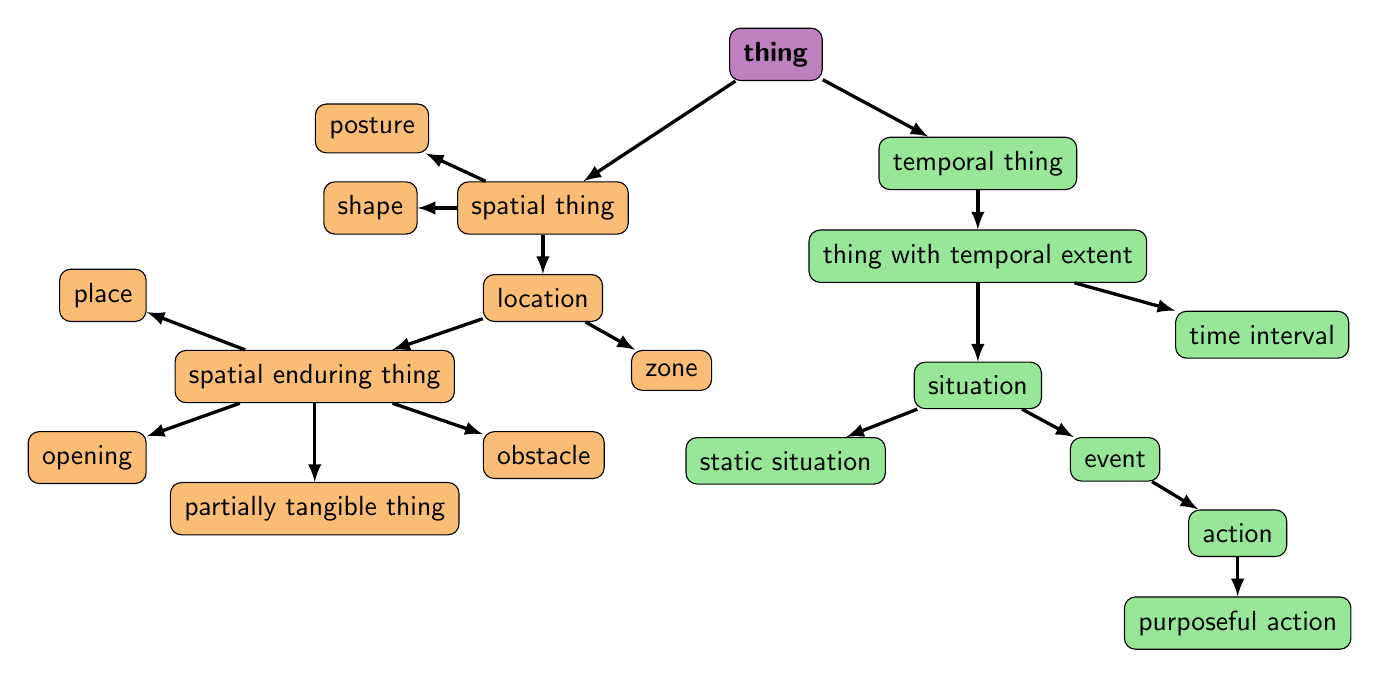
\begin{tikzpicture}[
    >=latex,
    every edge/.style={<-, draw, very thick},
    every node/.style={draw, font=\sf, node distance=0.5, rounded corners,
align=center, inner sep=5pt,fill=LimeGreen!50}]

    \node[fill=Purple!50] (thing) {\textbf{thing}};
    \node [fill=BurntOrange!50, node distance=1.8, below left=of thing](sthing) {spatial thing} edge (thing);
        \node [fill=BurntOrange!50, above left=of sthing] {posture} edge (sthing);
        \node [fill=BurntOrange!50, left=of sthing] {shape} edge (sthing);
        \node [fill=BurntOrange!50, below=of sthing] (location) {location} edge (sthing);
            \node [fill=BurntOrange!50, below right=of location] {zone} edge (location);
            \node [fill=BurntOrange!50, below left=of location] (set) {spatial enduring thing} edge (location);
                \node [fill=BurntOrange!50, below right=of set] {obstacle} edge (set);
                \node [fill=BurntOrange!50, below left=of set] {opening} edge (set);
                \node [fill=BurntOrange!50, below=1 of set] {partially tangible thing} edge (set);
                \node [fill=BurntOrange!50, above left=of set] {place} edge (set);

    \node [node distance=1, below right=of thing] (tthing) {temporal thing} edge (thing);
        \node [below=of tthing] (tte) {thing with temporal extent} edge (tthing);
            \node [below right=of tte] {time interval} edge (tte);
            \node [below=1 of tte] (sit) {situation} edge (tte);
                \node [below right=of sit] (evt) {event} edge (sit);
                    \node [below right=of evt] (act) {action} edge (evt);
                        \node [below=of act] {purposeful action} edge (act);
                \node [below left=of sit] {static situation} edge (sit);

\end{tikzpicture}
}

    \caption{The upper part of the {\sc Oro} common-sense conceptualization
    (TBox). These concepts are shared with the {\sc OpenCyc} upper-ontology.
    They relate to each other through `is-a' subsumption relations.}
    
    \label{fig|upper_tbox}
\end{figure}

\subsubsection{RDF as a Formalism for Semantics}

The {\sc Oro} server relies on Description Logics (OWL) to represent and
manipulate knowledge. Relying on RDF triples and Description Logics has advantages such as good
understanding of its trades-off, thanks to being widespread in the semantic Web
community, the availability of mature libraries to manipulate the ontology,
interoperability with several major on-line knowledge bases ({\sc
OpenCyc}, {\sc WordNet}, {\sc DBPedia} or {\sc RoboEarth}~\cite{Waibel2011} are
some examples), open-world reasoning, and the formal guarantee of decidability
(it is always possible to classify a Description Logics ontology).

It also has restrictions, both basic (the suitability of
Description Logics when reasoning on --typically non-monotonic-- commonsense
knowledge has been questioned) and practical: RDF triples imply binary
predicates, which constrains the expressiveness of the system or leads to
inconvenient reifications. Alternatives have been proposed (like {\sc
KnowRob}~\cite{Tenorth2009a}) that interleave RDF with more expressive logic languages
like {\sc Prolog} with however other limitations, like closed-world reasoning.

Classification performance is another issue: in our experience, an
ontology sized for a typical study (about 100 classes and 200 instances),
classification takes around 100ms, which leads to lags during
interactions.  Besides, the performances are difficult to predict: the insertion
of simple statements may indirectly change abruptly the logical
complexity of the whole knowledge model and lead to notable degradation of
classification time.

This knowledge model also largely excludes representation of continuous
phenomena (like time) or uncertain phenomena. When required (for instance for
action recognition), these are managed by dedicated components (like {\sc
Spark}, discussed in Section~\ref{sect|sit-ass}), and are not exposed at
the semantic level.

Alternative formalisms have been successfully investigated in robotics to
address some of these restrictions. \emph{Answer Set Programming} has been
used~\cite{Chen2010,Erdem2012} for instance to better supports non-monotonic
reasoning. We have also pointed in~\cite{lemaignan2015mutual} how modal logics like
the epistemic logics could be relevant to the particular field of social
human-robot interaction as they would allow for convenient representation of
alternative mental models. First-order logic and OWL ontologies have however
proved so far a simple, effective and sufficient symbolic framework for our
experimental applications. 

Incidentally, and because ontologies and RDF statements remain conceptually
simple (compared to full logical languages like {\sc Prolog} or modal logics),
their adoption has also effectively helped to grow awareness amongst colleagues
on the significance of the ``semantic level'' when developing new components
for the robot.

\subsubsection{The OpenRobots Ontology}

As previously said, the logical statements exchanged between the deliberative
components are organized within the {\sc Oro} knowledge base into an ontology.
The conceptualization (\ie the system of concepts or \emph{TBox}) of this
ontology is generally statically asserted, while the instantiation (the
\emph{ABox}) of the ontology is generally dynamically asserted at run-time, by
the other components.

The \emph{OpenRobots} common-sense ontology represents the statically asserted
part of the ontology. It has been designed from two requirements: beining
practical (\ie covering our experimental needs) and conforming as much as
possible to existing standards (in our case, the {\sc OpenCyc} upper
ontology~\cite{lenat1990cyc}).

This leads to a bidirectional design process: from \emph{bottom-up} regarding
the choices of concepts to model, \emph{top-down} regarding the upper part of
the taxonomy. This upper part of the ontology is pictured on
Figure~\ref{fig|upper_tbox}. All the classes visible in this figure belong to
the {\sc OpenCyc} namespace.

Aligning the upper part of the ontology on {\sc OpenCyc} (as done by other
knowledge representation systems, like {\sc KnowRob}~\cite{Tenorth2009a} or PEIS
K\&R~\cite{Daoutis2009}) has multiple advantages. First the design of this part
of the ontology is generally difficult: it pertains to abstract concepts whose
mutual relations comes to philosophical debates. The upper taxonomy of {\sc
OpenCyc} represents a relative consensus, at least within the semantic Web
community. Then, because it is a well established project with numerous links to
other on-line databases (like Wikipedia or WordNet), the reuse of key {\sc
OpenCyc} concepts ensures that the knowledge stored by the robot can be shared
or extended with well-defined semantics. The concept of \emph{Object} represents
a typical case of ambiguous meaning: in everyday conversation, an object is a
relatively small physical thing, that can be typically manipulated. A human is
not usually considered as an object. {\sc OpenCyc} however precisely defines an
object as anything at least \emph{partially tangible}. This includes obviously
the humans, and actually many other entities that would not be commonly said to
be objects (the Earth for instance).\footnote{In such cases of discrepancy
between {\sc OpenCyc} concepts and human terminology, we manually label the {\sc
OpenCyc} concepts with appropriate human names: for instance, the OpenRobots
Ontology associates the label ``\emph{object}'' to the concept
\concept{cyc:Artifact} instead of the concept \concept{cyc:PartiallyTangible}.
These labels are used in priority during the grounding of verbal interactions.}
Thus the importance of relying on well-defined and standard semantics to
exchange information between artificial systems in a non-ambiguous way.

Figure~\ref{fig|upper_tbox} also illustrates the fundamental disjunction
in the {\sc Oro} model between \emph{temporal} and \emph{spatial} entities (formally,
$(\text{\tt TemporalThing} \sqcap \text{\tt SpatialThing})^{\mathcal{I}} = \emptyset$, with
$\mathcal{I}$ the \emph{interpretation} of our model).

The class \concept{PurposefulAction} is the superset of all the actions that are
purposefully performed by the robot (or another agent). Actual actions (\ie
subclasses of \concept{PurposefulAction} like \concept{Give} or
\concept{LookAt}) are not initially asserted in the common-sense ontology. They
are instead added at run-time by the execution controller (in link with the
symbolic task planner) and the natural language processor based on what the
robot is actually able to perform and/or to interpret in the current context
(\ie the current robot configuration and the actions required by the scenario).
The set of actions that the robot can interpret usually closely resemble the
planning domain in use (\ie the set of tasks known to the symbolic task planner,
with their corresponding pre- and post-conditions).

The tree\footnote{While this subset of the ontology is a tree, it does not
generally have to be the case. In particular, the concept system (the
\emph{TBox}) of the {\sc Oro} common-sense ontology does not form a tree.} in
Figure~\ref{fig|upper_tbox} is not equally developed in every directions. For
example, the subclasses of \concept{PartiallyTangibleThing} (\ie what we
commonly call \emph{objects}) are shown in
Figure~\ref{fig|tangible_things_tbox}. Our `bottom-up'' design process of the
ontology is clearly apparent on this figure: only the subclasses relevant to the
context of service robotics in an human-like environment are explicitly stated.
For performance reasons as well as clarity, we have decided against an extended
conceptual coverage of what ``partially tangible things'' might be. We instead
opportunistically extend the common-sense knowledge when required by studies.


\begin{figure}
    \centering

\resizebox{0.5\textwidth}{!}{%
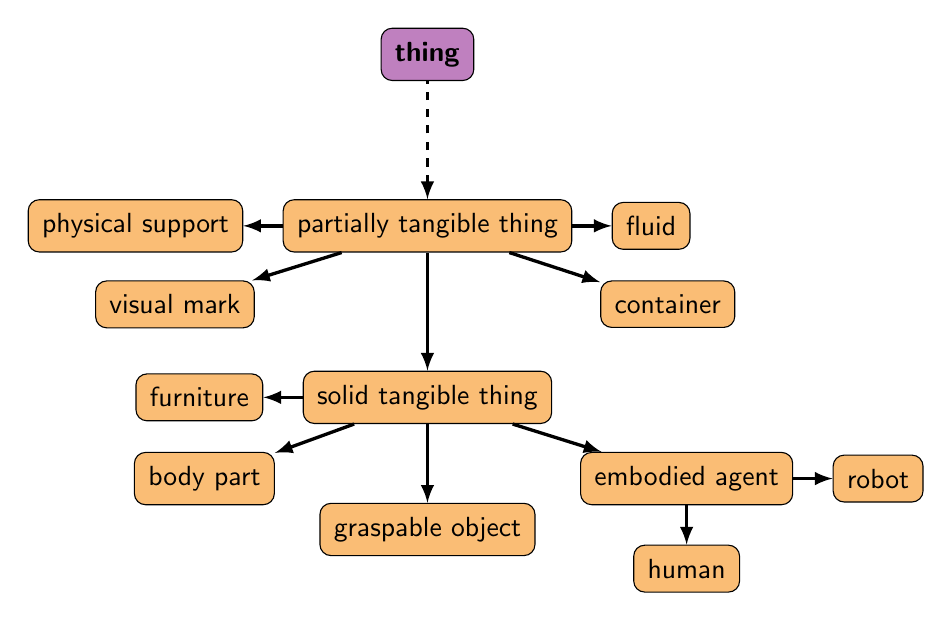
\begin{tikzpicture}[
    >=latex,
    every edge/.style={<-, draw, very thick},
    every node/.style={draw, font=\sf, node distance=0.5, rounded corners,
align=center, inner sep=5pt,fill=BurntOrange!50}]

    \node[fill=Purple!50] (thing) {\textbf{thing}};
    \node [below=1.5 of thing] (ptt) {partially tangible thing} edge[dashed] (thing);
        \node [left=of ptt] {physical support} edge (ptt);
        \node [below left=of ptt] {visual mark} edge (ptt);
        \node [below right=of ptt] {container} edge (ptt);
        \node [right=of ptt] {fluid} edge (ptt);
        \node [below=1.5 of ptt] (stt) {solid tangible thing} edge (ptt);
            \node [below=1 of stt] {graspable object} edge (stt);
            \node [below left=of stt] {body part} edge (stt);
            \node [left=of stt] {furniture} edge (stt);
            \node [below right=of stt] (ea) {embodied agent} edge (stt);
                \node [below=of ea] {human} edge (ea);
                \node [right=of ea] {robot} edge (ea);

\end{tikzpicture}
}
    \caption{Subclasses of \concept{PartiallyTangibleThing} explicitly stated in the
    OpenRobots Ontology.}
    \label{fig|tangible_things_tbox}
\end{figure}

Lastly, the {\sc Oro} common-sense ontology contains several rules and class
expressions that encode non-trivial inferences. The definition of
\concept{Bottle} as found in the {\sc Oro} ontology is a typical example:
$$
\text{\tt Bottle} \equiv \text{\tt Container} \wedge 
                         \text{\tt GraspableObject} \wedge
                         \text{\tt hasShape} \in \text{\tt CylinderShape}^{\mathcal{I}} \wedge
                         \text{\tt hasMainDimension} \in [0.1, 0.3]
$$

If a human informs the robot that a given object is indeed a bottle, the robot
derives more information on the object. Conversely, if the human affirms that
``a car is a bottle'', the reasoner may detect logical contradictions (like
inconsistent sizes) and reject the assertion. The {\sc Dialogs} module relies
on such logical consistency checks when processing natural language inputs,
both to ensure that the verbal input has been correctly acquired and parsed,
and also to verify that what the human says is logically consistent.  We
further discuss the strengths and weaknesses of this knowledge framework in
Section~\ref{krs-discussion}.

\subsection{Symbol Grounding}

\emph{Grounding} (also called \emph{anchoring} when specifically referring to
the building of links between \emph{percepts} and \emph{physical
objects}~\cite{Coradeschi2003}) is the task consisting in building and
maintaining a bi-directional link between sub-symbolic representations (sensors
data, low-level actuation) and symbolic representations that can be manipulated
and reasoned about~\cite{Harnad1990}. This represents an important cognitive
skill, in particular in the human-robot interaction context: in that case, the
link that the robot has to establish between percepts and symbols must
map as well as possible to the human representations in order to effectively
support communication.

\emph{Symbol grounding} connects hence the knowledge model to the perception and
actuation capabilities of the robot. The different components that we have
mentioned so far provide a bottom-up grounding process: geometric reasoning and
dialogue processing modules constantly build and push new symbolic contents
about the world to the knowledge base where it becomes accessible to decisional
layers. We detail this process in the next sections. 


%%%%%%%%%%%%%%%%%%%%%%%%%%%%%%%%%%%%%%%%%%%%%%%%%%%%%%%%%%%%%%%%%%%%%%%%%%%%%%%%
\section{Cognitive Skills}
\label{sec:impl}

The previous section has provided an overview of our cognitive architecture
as well as the associated knowledge model. We discuss in this section its
building blocks. Each of these components have connections to several
others, and Figure~\ref{fig|archi} can be referred to as a guide.

\begin{inparaenum} We call \emph{cognitive skills} the
deliberative behaviours that are \item \emph{stateful}, \ie keeping track of
previous states is typically needed for the component to perform adequately;
\item \emph{amodal} in that the skill is not inherently bound to a specific
perception or actuation modality; \item manipulate \emph{explicit semantics},
typically by the mean of symbolic reasoning; \item operate at the
    \emph{human-level}, \ie are legible to the humans, typically by acting at
similar levels of abstraction.\end{inparaenum}

We present first the main \emph{internal} cognitive capabilities, implemented in
the {\sc Oro} knowledge base itself, and then discuss successively the situation
assessment module {\sc Spark}, the dialogue processor {\sc Dialogs}, the
symbolic task planner HATP, and finally the main features of our execution
controllers {\sc Shary} and {\sc pyRobots}. Note that greater details on each of
these modules can be found in their respective publications (the corresponding
references are provided hereafter).

\subsection{Internal Cognitive Skills}
\label{sect|intern}

We call \emph{internal} those cognitive capabilities that are tightly bound to
the knowledge model, and hence implemented directly within the {\sc Oro} server.
We present here three of them: \emph{reasoning}, \emph{theory of mind} modelling
and our (naive) approach to \emph{memory management}.

\subsubsection{Symbolic Reasoning}
\label{reasoning}

As mentioned in the previous section, we use the Pellet open-source reasoner to
reason on the knowledge base. It supports several standard inference processes:
consistency checking, concept satisfiability, classification and realisation
(computation of the most specific classes that a concept belongs to). In
case of logical inconsistency, the reasoner can also provide explanations (we
currently only use them for debugging purposes).

Besides, {\sc Oro} server implements several algorithms (presented
in~\cite{Ros2010b}) to identify
similarities and differences between concepts (classes or
instances): the \emph{Common Ancestors} algorithm, useful to
determine the most specific class(es) that include a given set of individuals;
the \emph{First Different Ancestors} algorithm that returns what can be
intuitively understood as the most generic types that \emph{differentiate} two
concepts; and \emph{clarification} and \emph{discrimination} algorithms that
play a key role in the process of \emph{interactive grounding} of the semantics
of concepts (we discuss this process in section~\ref{sect|com}). Clarification
and discrimination algorithms are based on what we call \emph{descriptors}, \ie
properties of individuals, either statically asserted in the common-sense
ontology, acquired by the robot through perception or pro-active questioning of
the human partner, or derived from other reasoning algorithms like the
\emph{Common Ancestors} and \emph{Different Ancestors}. The
\emph{discrimination} algorithm consists then in looking for discriminants, \ie
descriptors that allow a maximum discrimination among a set of individuals.

\subsubsection{Theory of Mind}
\label{sect|tom}

Theory of Mind (originally defined in~\cite{Premack1978}) is the cognitive
ability that allows a subject to represent the mental state of another
agent, possibly including knowledge that contradicts the subject's own model: for
example, a book can be at the same time \emph{visible} for agent A, and \emph{not
visible} for agent B. Children develop this skill, which is essential to understand others' perspectives during
interactions, around the age of three~\cite{perner2012infants}. 

From the point of view of interactive robotics, it supposes the robot ability to
build, store and retrieve separate models of the beliefs of the humans it
interacts with.  Our knowledge base implements such a mechanism: when the robot
detects that a new human has appeared, it initialises a new independent
knowledge model (an ontology) for this human agent. All the ontologies that are
created share the same common-sense knowledge, but rely on the estimation of the
robot of each agent's perspective for their actual instantiation. For example,
the robot may (geometrically) compute that the book is in its own field of view,
but not in the human one (the detail of this computation, called
\emph{perspective taking}, is discussed in the next section). The robot updates
accordingly the two knowledge models it maintains: the \concept{robot} model is
updated with the fact \stmt{book isVisible true}, while the \concept{human}
model is updated with \stmt{book isVisible false}. These two logical statements
are simultaneously asserted, yet contradict when taken together. Since the two
knowledge models are realized as two independent ontologies, the contradiction
does not actually occur and both the models remain logically consistent.

One classical application of this cognitive skill is the so-called
\emph{False-Belief} experiment (also known as the \emph{Sally and Anne}
experiment, introduced by~\cite{wimmer1983beliefs} from an original
experimental setting by~\cite{baron1985does}): a child is asked to watch a scene where two
people, A and B, manipulate objects. At some point, A leaves and B hides away one
object. When A comes back, we ask the child ``where do you think A will
look for the object?''. Before acquiring a theory of mind, children are not
able to separate their own (true) model of the world (where they know that
the object was hidden) from the model of A, which contains \emph{false
beliefs} on the world (A still thinks the object is at its original
position since he did not see B hiding it in a new place). Using separate knowledge models
in the knowledge base, we have been able to replicate this experience with
our robots~\cite{warnier2012when}, in a manner similar to Breazeal
\etal\cite{breazeal2009embodied}.

\subsubsection{Working Memory}
\label{memory}

Memory has been studied at length in the cognitive psychology and
neuro-psychology communities: the idea of \emph{short-term} and \emph{long-term}
memory is due to Atkinson and Shiffrin~\cite{Atkinson1968};
Anderson~\cite{Anderson1976} proposes to split memory into \emph{declarative}
(explicit) and \emph{procedural} (implicit) memories; Tulving~\cite{Tulving1985}
organises the concepts of \emph{procedural}, \emph{semantic} and \emph{episodic}
memories into a hierarchy. Short-term memory is eventually refined with the
concept of \emph{working memory} by Baddeley~\cite{Baddeley2010}.  In the field
of cognitive architectures, the {\sc Soar} architecture~\cite{Lehman2006} is one
of those that try to reproduce a human-like memory organisation. The GLAIR
cognitive architecture~\cite{Shapiro2009} also has a concept of long term/short
term and episodic/semantic memories.

It is worth emphasising that while memory is commonly associated with the process of
forgetting facts after a variable amount of \emph{time}, it actually covers
more mechanisms that are relevant to robotics, like priming
(concept pre-activation triggered by a specific
context~\cite{baxter2012modelling}) or reinforcement learning.

The {\sc Oro} server features a mechanism to mimic only minimalistic forms of memory
families.  When new statements are inserted in the knowledge base, a
\emph{memory profile} is attached to them.  Three such profiles are
predefined: {\it short term}, {\it episodic} and {\it long term}. They are
currently attached to different lifetime for the statements (respectively 10
seconds, 5 minutes and no time limit). After this duration, the statements are
automatically removed.

This approach is limited. In particular, \emph{episodic} memory should primarily
refer to the semantics of the statements (that is expected to be related to an
event) and not to a specific lifespan.

We rely however on this mechanism in certain cases: some modules
like the natural language processor use the {\it short term} memory profile to
mark concepts that are currently manipulated by the
robot as \emph{active concepts}: if a human asks the robot ``Give
me all red objects'', the human, the \concept{Give} action, and each red
objects that are found are successively marked as \emph{active concepts} by
inserting statements such as \stmt{human type ActiveConcept} in the short-term
memory (which can be considered, in this case, to be a working memory).
Likewise, recently seen or updated geometric entities are flagged as
\concept{ActiveConcept}. We use this feature during dialogue disambiguation for
instance. On the other hand, our perception layer does not make use of this
mechanism: as described in the next section, the environment model of the robot
is continuously updated and the derived symbolic knowledge is therefore
transient: it lasts only as long as the environment remains in the same state.


\subsection{Acquiring and Anchoring Knowledge in the Physical World}
\label{sect|sit-ass}

\begin{figure}
\centering
\resizebox{0.8\textwidth}{!}{%
\begin{tikzpicture}[
        >=latex,
        box/.style={draw,rectangle, dotted, minimum width=#1, minimum height=3.8cm},
        box/.default={4cm},
        every edge/.style={draw, ultra thick},
        every node/.style={align=center}]

    %\draw[step=1cm, draw=black!20] (-10,-5) grid (10,5);

    \node[draw=none] at (0,-1.5) {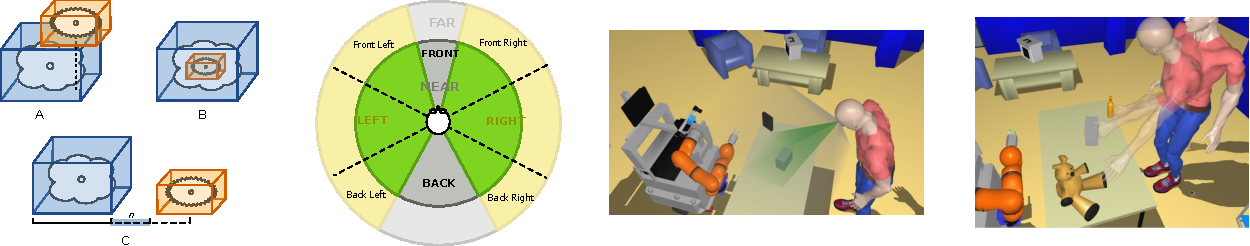
\includegraphics[width=1.\columnwidth]{spark-oro-notext.pdf}};

    \node[box=16cm, minimum height=5.3cm, solid, thick, rounded corners] at (0,1.8) (oro) {};
    \node at (0,4.2) {\sc \Large oro-server};

    \node[anchor=south] at (-4.6,2.4) {Description Logics \\ (Open World assumption)};
    \node[box=3.7cm] at (-4.6,1.9) (owl) {};
    \node[anchor=south] at (-1,2.4) {Multiple simultaneous \\ symbolic models};
    \node[box=3.3cm] at (-1,1.9) (multi) {};
    \node[anchor=south] at (2.1,2.4) {Bio-inspired \\ memory};
    \node[box=2.7cm] at (2.1,1.9) (mem) {};
    \node[anchor=south] at (5,2.4) {Discrimination \& \\ categorization};
    \node[box=3cm] at (5,1.9) (disc) {};

    \node at (-3,-0.4) {{\it OWL store:} OpenJena};
    \node at (3,-0.4) {{\it Reasoner:} Pellet};

    %%%%%%%%%%%%%%%%%%%%%%%%%%%%%%%%%%%%%%%%%%%%%%%%%%%%%%%%%%%%%%%%%%%%%%%%%%%%%%%%%%%

    \node[box=18cm, minimum height=4.5cm, dotted, thick, rounded corners] at (0,-4.2) (spark) {};
    \path (spark.north) edge[->] node[align=left,anchor=west] {Symbolic\\facts} (oro.south);

    \node[anchor=north] at (-6.5,-5.3) {a) Agent-independent\\(allocentric)
        spatial relations};
    \node[anchor=north] at (-2.1,-5.3) {b) Agent-dependent\\(egocentric) spatial
        relations};
    \node[anchor=north] at (1.6,-5.3) {c) Visibility/Pointing};
    \node[anchor=north] at (6.5,-5.3) {d) Reachability};

\end{tikzpicture}
}
    \caption{Functional overview of knowledge base ({\sc Oro} server, top part)
    and the geometric situation assessment module (\emph{{\sc Spark}}, bottom
    part). {\sc Spark} computes symbolic relationships between objects and
    agents, and exports them to the knowledge base.}

        \label{fig|spark-oro}
\end{figure}

Anchoring perceptions in a symbolic model requires perception abilities and
their symbolic interpretation. We call \emph{physical situation assessment} the
cognitive skill that a robot exhibits when it assesses the nature and content of its
surroundings and monitors its evolution.

Numerous approaches exist, like amodal (in the sense of modality-independent)
\emph{proxies}~\cite{Jacobsson2008}, grounded amodal
representations~\cite{Mavridis2006}, semantic
maps~\cite{Nuechter2008, Galindo2008,Blodow2011} or affordance-based planning
and object classification~\cite{Lorken2008, Varadarajan2011}.

%Spatial reasoning~\cite{O'Keefe1999} is a field in its own right, and has been
%used for natural language processing for applications such as direction
%recognition ~\cite{Kollar2010,Matuszek2010} or language
%grounding~\cite{Tellex2010}.~\cite{Skubic2004} present a spatial reasoner
%integrated in a robot which computes symbolic positions of objects.


We rely on a dedicated geometric and temporal reasoning module called {\sc
Spark} (\emph{SPAtial Reasoning \& Knowledge}, presented in~\cite{Sisbot2011}).
It is a situation assessment reasoner that generates symbolic knowledge from the
geometry of the environment with respect to relations between objects, robots
and humans (Figures~\ref{fig|spark-oro} and~\ref{fig:sparkSubfigures}), also
taking into account the different perspective that each agent has on the
environment.  {\sc Spark} embeds an \emph{amodal} (as defined by Mavridis and
Roy in~\cite{Mavridis2006}: the different perceptual modalities are abstracted
away into a blended spatial model) geometric model of the environment that
serves both as basis for the fusion of the perception modalities and as bridge
with the symbolic layer. This geometric model is built from 3D CAD models of the
objects, furnitures and robots, and full body, rigged models of humans
(Figure~\ref{fig:sparkScreenshot}).  It is updated at run-time by the robot's
sensors (usually, a combination of vision-based tracking of 2D fiducial markers
to identify and localize objects, and Kinect-based skeleton tracking of humans,
optionally assisted by motion capture to accurately track the head motion, which
is required to compute what the human is looking at).

{\sc Spark} runs and continuously updates the knowledge base at about 10Hz. At
each step, it re-computes spatial relations and affordances for the whole scene,
and send the delta (new relations and relations that do not hold anymore) to the
knowledge base. This approach may raise scalability concerns (we did not however
hit major performance issues in our constrained scenarios) as well as prevent
reasoning on the situation history, but simplifies the management of the
dynamics of the knowledge (\emph{When do I discard outdated knowledge?  When do
I update it?}). Since it is equivalent to a reset of the reasoner domain, it
also essentially nullifies issues linked to non-monotonic reasoning
(see~\cite{McCarthy2007} for a discussion on that question).


\begin{figure*}[ht!]
   \begin{center}
%
       \subfigure[Physical setting]{%
           \label{fig:wuweiPhoto}
           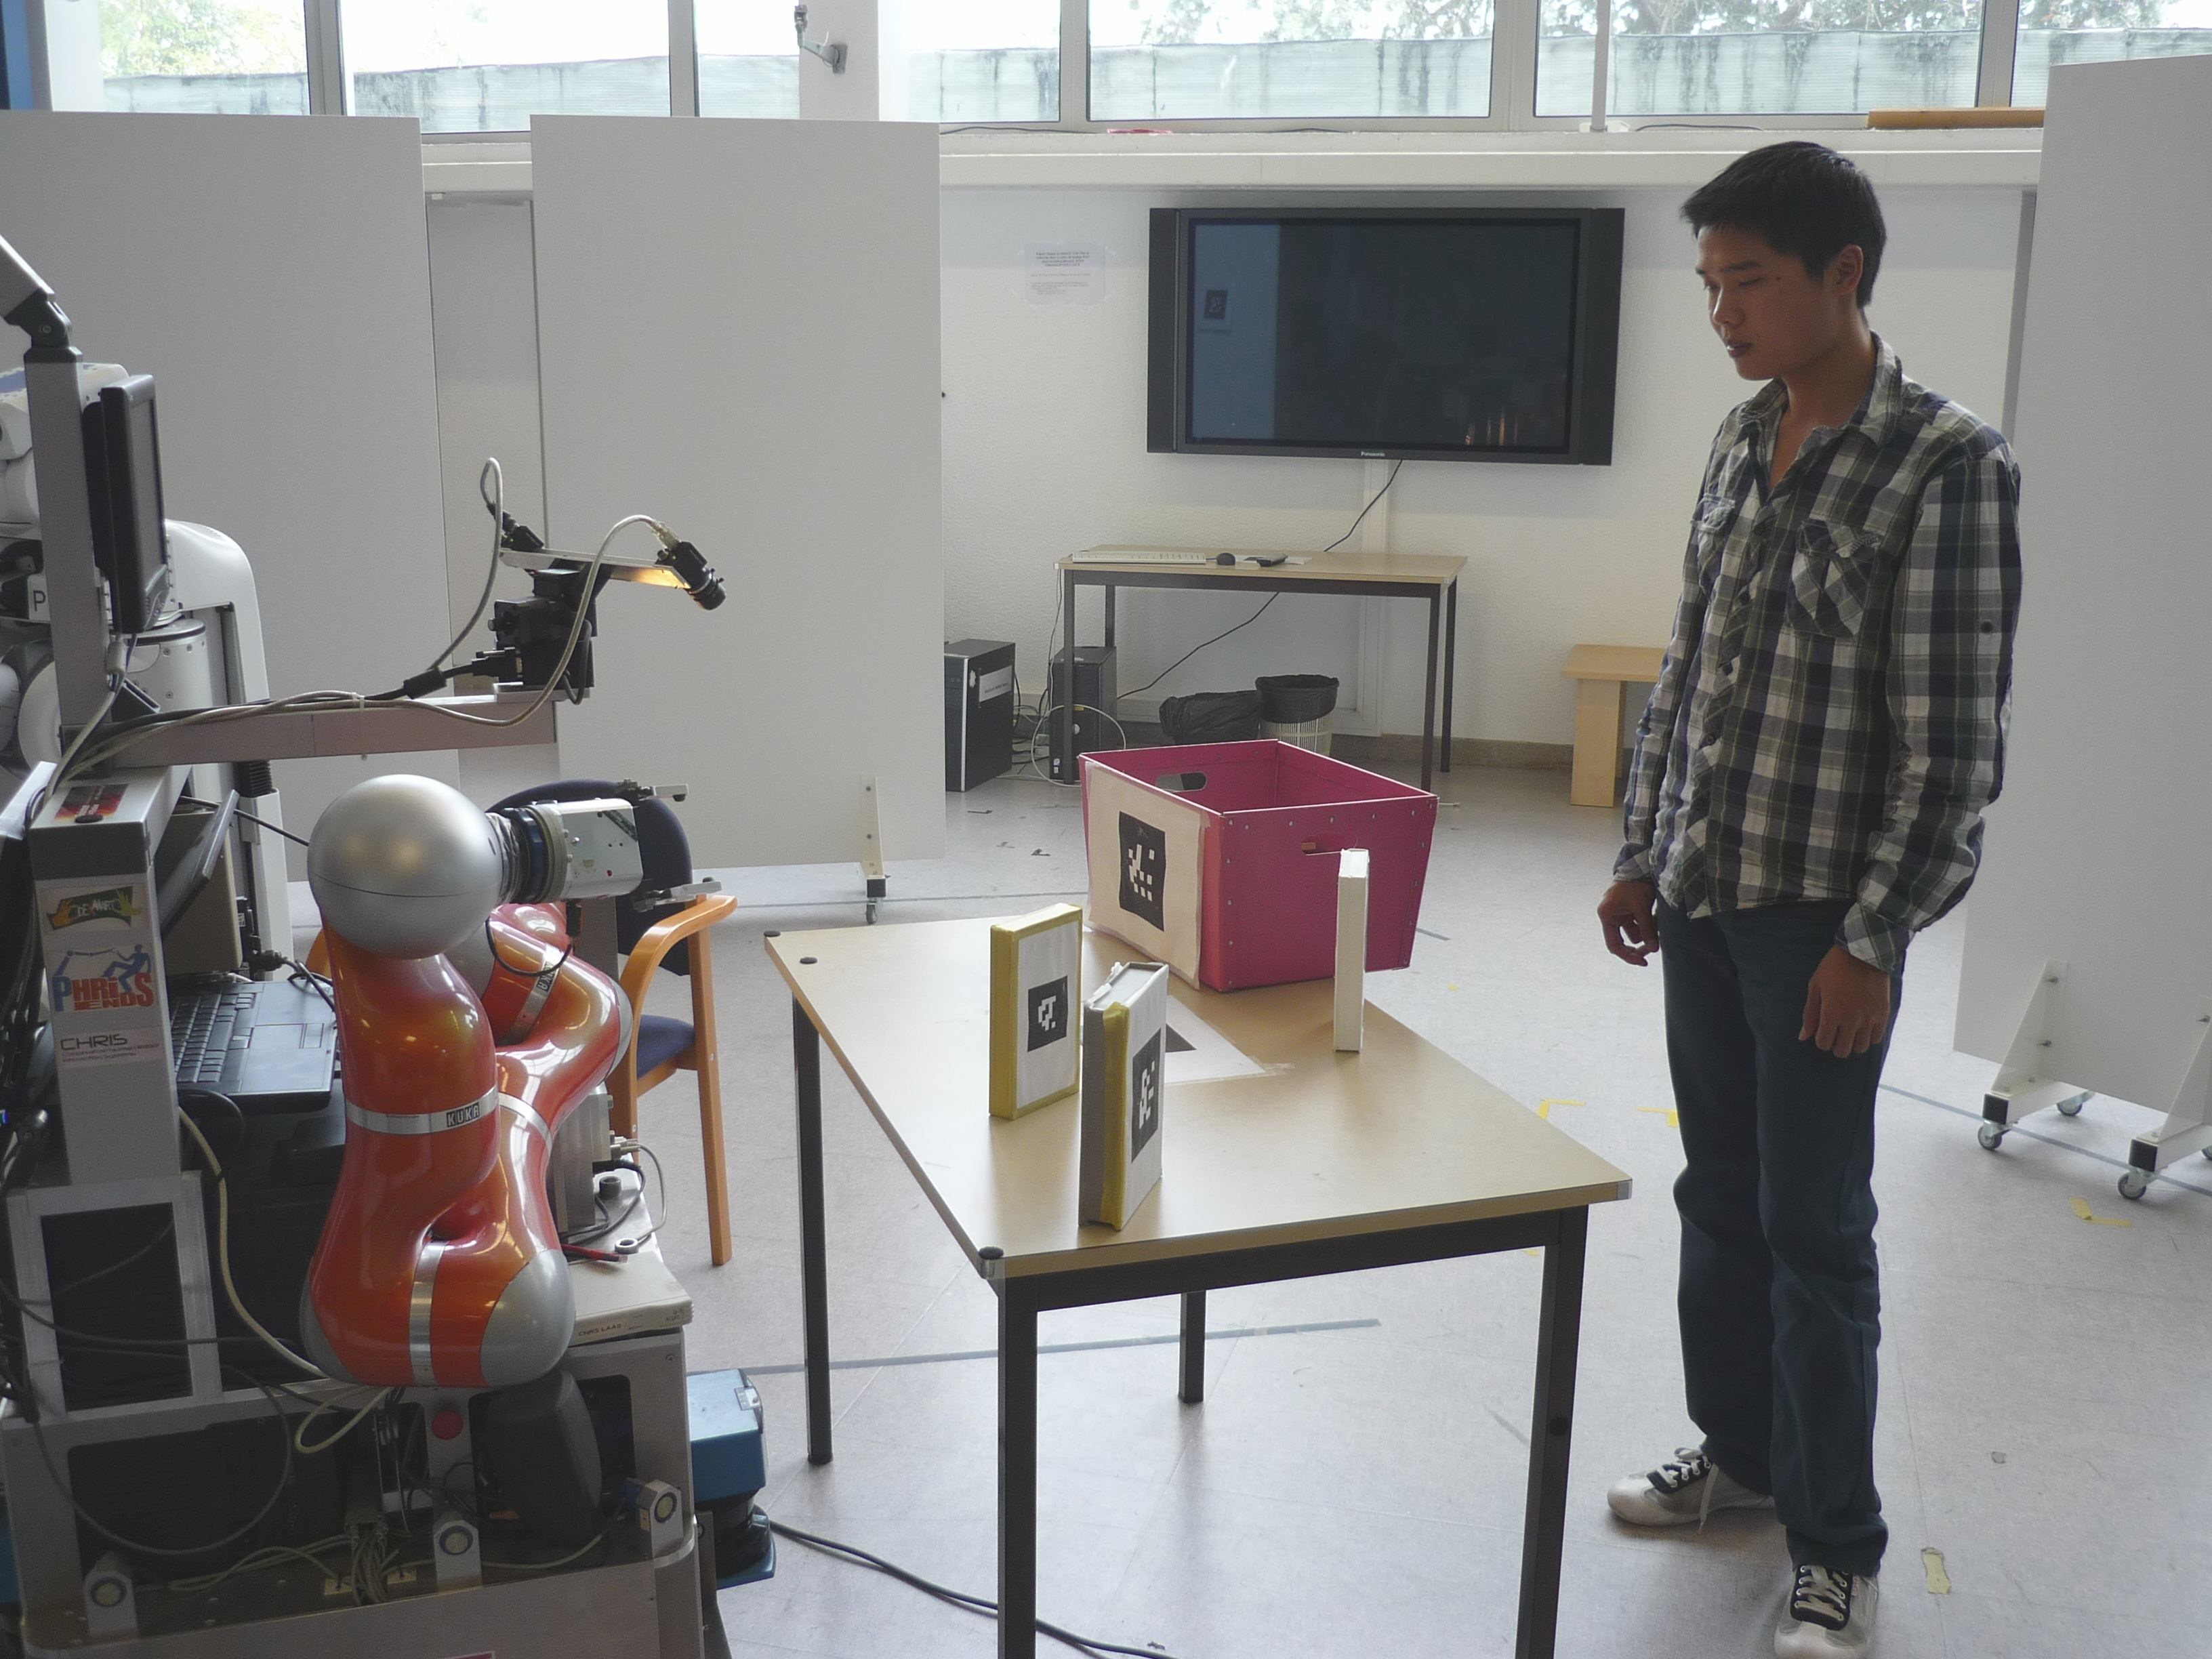
\includegraphics[width=0.5\textwidth]{etat2-P1010769_brightened-v2.jpg}
       }%
       \subfigure[Corresponding 3D model view]{%
          \label{fig:sparkScreenshot}
          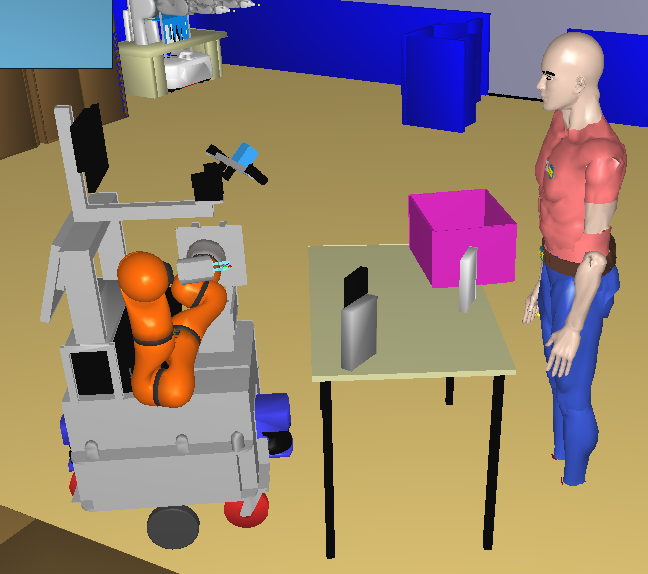
\includegraphics[width=0.43\textwidth]{etat2_photo.png}
       }\\ %  ------- End of the first row ----------------------%
%
   \end{center}

   \caption{Test setup involving videotapes boxes that are manipulated, with other
       objects acting as supports or containers. After identification and
       localisation of the set of objects (using fiducial markers) and
       acquisition of the position and posture of the human partner (using
       skeleton tracking), the robot is able to compute that two tapes only are
       reachable by itself: the black and grey (in the 3D model) tapes.  The
       third tape and the pink container box are only reachable by the human. This
       physical situation is transformed by {\sc Spark} into the set of facts 
       presented in Table~\ref{table|beliefsfig7}.  }%
        
 \label{fig:sparkSubfigures}

\end{figure*}

\begin{table}
\begin{center}
    \subfigure{
\begin{tabular}{l}
\hline
Robot's beliefs about itself (\emph{robot's model})\\
\hline
\hspace{0.7cm}\stmt{PINK\_BOX isReachable {\bf false}}\\
  \hspace{0.7cm}\stmt{WHITE\_TAPE isReachable {\bf false}}\\
  \hspace{0.7cm}\stmt{BLACK\_TAPE isReachable {\bf true}}\\
  \hspace{0.7cm}\stmt{GREY\_TAPE isReachable {\bf true}}\\
  \hspace{0.7cm}\stmt{WHITE\_TAPE isVisible true}\\
  \hspace{0.7cm}\stmt{BLACK\_TAPE isVisible true}\\
  \hspace{0.7cm}\stmt{GREY\_TAPE isVisible true}\\
  \hspace{0.7cm}\stmt{WHITE\_TAPE isOn TABLE}\\
  \hspace{0.7cm}\stmt{BLACK\_TAPE isOn TABLE}\\
  \hspace{0.7cm}\stmt{GREY\_TAPE isOn TABLE}\\
\hline
\end{tabular}
}\hspace{1em}%
\subfigure{
\begin{tabular}{l}
\hline
Robot's beliefs about the human (\emph{human's model})\\
\hline
  \hspace{0.7cm}\stmt{PINK\_BOX isReachable {\bf true}}\\
  \hspace{0.7cm}\stmt{WHITE\_TAPE isReachable {\bf true}}\\
  \hspace{0.7cm}\stmt{BLACK\_TAPE isReachable {\bf false}}\\
  \hspace{0.7cm}\stmt{GREY\_TAPE isReachable {\bf false}}\\
  \hspace{0.7cm}\stmt{WHITE\_TAPE isVisible true}\\
  \hspace{0.7cm}\stmt{BLACK\_TAPE isVisible true}\\
  \hspace{0.7cm}\stmt{GREY\_TAPE isVisible true}\\
  \hspace{0.7cm}\stmt{WHITE\_TAPE isOn TABLE}\\
  \hspace{0.7cm}\stmt{BLACK\_TAPE isOn TABLE}\\
  \hspace{0.7cm}\stmt{GREY\_TAPE isOn TABLE}\\ 
 \hline
\end{tabular}
}
\end{center}
\caption{Symbolic facts computed from the situation depicted in
Figure~\ref{fig:sparkSubfigures}. Note how reachability differs for the two
agents.}

\label{table|beliefsfig7}
\end{table}

\subsubsection{Building an Agent-Aware Symbolic Model of the Environment}
\label{sect|situ}

\paragraph{Perspective Taking} \emph{Visual} perspective taking refers to the
ability for visually perceiving the environment from another person's point of view.
This ability allows us to identify the objects in situations where the visual
perception of one person differs from the other one. In developmental
psychology, one typical example consists of two similar objects in a room (\eg
two balls) where both are visible for the child, but only one is visible for
the adult. Thus, when the adult asks the child to hand over ``the ball'', the
child is able to correctly identify which ball the adult is referring to (\ie
the one visible from the adult point of view), without asking~\cite{Moll2006}.
Our architecture endows the robot with such a cognitive skill.

\emph{Spatial} perspective taking refers to the qualitative spatial location of
objects (or agents) with respect to a frame (\eg \emph{the keys on my left}).
Based on this frame of reference, the description of an object
varies~\cite{Marin2008}. Humans mix perspectives frequently during interaction.
This is more effective than maintaining a consistent one, either because the
(cognitive) cost of switching is lower than remaining with the same
perspective, or if the cost is about the same, because the spatial situation
may be more easily described from one perspective rather than
another~\cite{Tversky1999}. Ambiguities arise when one speaker refers to an
object within a reference system (or changes the reference system, \ie switches
perspective) without informing his/her partner about it~\cite{Breazeal2006,
Ros2010}. For example, the speaker could ask for the ``keys on the left''.
Since no reference system has been given, the listener would not know where
exactly to look.  However, asking for ``the keys on your left'' gives enough
information to the listener to understand where the speaker is referring to. On
the contrary, when using an exact, unambiguous term of reference to describe a
location (\eg. ``go north'') no ambiguity arises.
In {\sc Spark}, agent-dependent spatial relations are computed from the frame of
reference of each agent.

\paragraph{Symbolic Locations}

Humans commonly refer to the positions of objects with symbolic descriptors
(like \emph{on}, \emph{next to}...) instead of precise, absolute positions
(qualitative spatial reasoning). These type of descriptors have been studied in the context of language grounding
\cite{O'Keefe1999,Matuszek2010,Regier2001,Kelleher2006,Blisard2005}.  {\sc
Spark} distinguishes between agent-independent symbolic locations (allocentric
spatial relations) and agent-dependent, relative locations (egocentric spatial
relations).

{\sc Spark} computes three main agent-independent relations~\cite{Sisbot2011}
based on the bounding box and centre of mass of the objects
(Figure~\ref{fig|spark-oro}\emph{a}): \concept{isOn} holds when an object $O_1$
is on another object $O_2$, and is computed by evaluating the centre of mass of
$O_1$ according to the bounding box of $O_2$.  \concept{isIn} evaluates if an
object $O_1$ is inside another object $O_2$ based on their bounding boxes
$BB_{O_1}$ and $BB_{O_2}$.  \concept{isNextTo} indicates whether an object $O_1$
is next to another object $O_2$. We do not use a simple distance threshold to
determine if two objects are next to each other since the relation is highly
dependent on the dimensions of the objects. For instance, the maximum distance
between large objects (\eg two houses) to consider them as being next to each
other is much larger than the maximum distance we would consider for two small
objects (\eg two bottles). Thus, the distance threshold is scaled with the
objects' size. {\sc Spark} also compute symbolic facts related to agent
independent world dynamics.  The predicate \concept{isMoving} states, for each
tracked entity, whether it is currently moving or not.

Many other topological relations are dependent from the observation point
(egocentric perspective).  The predicate \concept{hasRelativePosition}
represents such spatial relations between agents and objects that are agent
dependent.  We compute these spatial locations by dividing the space around the
referent (an agent) into $n$ regions based on arbitrary angle values relative to
the referent orientation (Figure~\ref{fig|spark-oro}\emph{b}).  For example, for
$n = 4$ we would have the space divided into \emph{front, left, right} and
\emph{back}. Additionally, two proximity values, \emph{near} and \emph{far}, are
also considered. The number of regions and proximity values can be chosen
depending on the context where the interaction takes place.

Through perspective taking, {\sc Spark} computes for each agent a symbolic
description of the relative positioning of objects in the environment.
Table~\ref{facts} summarises all the symbolic spatial relations computed by {\sc
Spark}.

\subsubsection{Building a Model of Agents}
\label{sect|grounding_agents}

Building a grounded symbolic model of the physical environment does not suffice
in general to fully ground the human-robot interaction, and a model of the
current capabilities of the agents interacting with the robot is also required.

{\sc Spark} computes the following capabilities from the perspectives of each agent:

\begin{itemize}

\item \emph{Sees}: this relation describes what the agent can see, \ie what is
    within its field of view (FOV). In our current implementation, this
    affordance is computed by dynamically placing an OpenGL camera at the
    location of the eyes and running occlusion checks from it.  In
    Figure~\ref{fig|spark-oro}\emph{c} the field of view of a person is
    illustrated with a grey cone (the wider one). While he is able to see the two
    small boxes on the table in front of him, the big box on his right is out of
    his FOV, and therefore, he is not able to see it. 

    Besides, {\sc Spark} also computes the \concept{seesWithHeadMovement}
    relation by simulating a small left-right rotation of the head. It
    represents what an agent \emph{could} see with a minimal effort.
    

\item \emph{Looks At}: this relation corresponds to what the agent is focused
    on, \ie where its focus of attention is directed. This model is based on a
    narrower field of view, the field of attention (FOA).
    Figure~\ref{fig|spark-oro}\emph{c} shows the field of attention
    of a person with a green cone (the narrower one). In this example only the grey
    box satisfies the \concept{looksAt} relation.


\item \emph{Points At} holds when an object is pointed at by an agent.
    This relation is computed by placing a virtual camera on the hand, aligned
    with the forearm. \concept{pointsAt} is typically used during dialogue
    grounding, for instance when one of the agents is referring to an object
    saying ``this'' or ``that'' while pointing at it.
\end{itemize}

To ensure a sufficiently stable recognition, these three capabilities are post-filtered
with an hysteresis function at the geometric level.

\begin{itemize}
\item \emph{Reachable} enables the robot to estimate the agent's ability to
    reach for an object, which is instrumental for effective social task
    planning. For example, if the human asks the robot to give her an object,
    the robot must compute a transfer point where she is able to get the
    object afterwards.  Reachability is computed for each agent (human or robot) based on
    Generalised Inverse Kinematics and collision detection. More than that, our robot is able 
    to compute an estimate of the effort needed by an agent to reach an object\cite{pandey2013affordance}.

\end{itemize}

Table~\ref{facts} also lists these abilities, along with the admissible classes
for the subjects and objects of the statements.

\renewcommand{\concept}[1]{{\scriptsize \texttt{#1}}}
\begin{table}[h]
    \centering
    \begin{tabular}{p{1.5cm}lp{2cm}p{5cm}}
    \textbf{Subject} & \textbf{Predicate} & \textbf{Object} & \emph{Notes} \\ 
    \hline
	 \concept{Location} & \concept{isAt} $\equiv$ \concept{cyc:objectFoundInLocation}  &  \concept{Location} & \\ 
	 &  $\rightarrow$ \concept{isOn} $\equiv$ \concept{cyc:above\_Touching}  &  & \\ 
	 &  $\rightarrow$ \concept{isIn}  &  & \\ 
	 &  $\rightarrow$ \concept{isNextTo}  & &  \\ 
	 \concept{Location}  & \concept{isAbove} $\equiv$ \concept{cyc:above-Generally}  &  \concept{Location}  &  inverse of \concept{isBelow} \par \concept{isOn} $\Rightarrow$ \concept{isAbove}\\ 
	 \concept{Location}  & \concept{isBelow}  & \concept{Location}  &  inverse
	of \concept{isAbove} \\
	\hline
	 \concept{Location}  & \concept{hasRelativePosition}  & \concept{Location} & \\ 
	 & 	$\rightarrow$ \concept{behind} $\equiv$ \concept{cyc:behind-Generally}  &  & inverse of \concept{inFrontOf}  \\ 
	 &  $\rightarrow$ \concept{inFrontOf} $\equiv$ \concept{cyc:inFrontOf-Generally}  & 	 & 	 inverse of \concept{behind}  \\ 
	 &  $\rightarrow$ \concept{leftOf}  &  &  inverse of \concept{rightOf} \\ 
	 &  $\rightarrow$ \concept{rightOf}  & 	 & 	 inverse of \concept{leftOf}  \\ 
	 \concept{Object}  & \concept{cyc:farFrom}  &  \concept{Agent} & \\ 
	 \concept{Object}  & \concept{cyc:near}  &  \concept{Agent} & \\

		\hline
		 \concept{Agent}  & \concept{looksAt}  & \concept{SpatialThing} \\
		 \concept{Agent}  & \concept{sees}  &  \concept{SpatialThing}  &    \\ 
		 \concept{SpatialThing}  & \concept{isInFieldOfView}  & \concept{xsd:boolean}  & \par \tiny \concept{myself sees *} $\Leftrightarrow$ \concept{* isInFieldOfView true} \\ 
		 \concept{Agent}  & \concept{pointsAt} $\equiv$ \concept{cyc:pointingToward}  & \concept{SpatialThing} \\ 
		 \concept{Agent}  & \concept{focusesOn}  &  \concept{SpatialThing}  &  \par \tiny \concept{looksAt} $\wedge$ \concept{pointsAt} $\Leftrightarrow$ \concept{focusesOn} \\
		\concept{Agent} & \concept{seesWithHeadMovement} &  \concept{SpatialThing} \\
        \concept{Agent} & \concept{canReach} &  \concept{Object} & \\ 
        \concept{Object} & \concept{isReachable} &  \concept{xsd:boolean} & \par \tiny \concept{myself canReach *} $\Leftrightarrow$ \concept{* isReachable true} \\ 

	\end{tabular}

    \caption{List of statements describing agent-independent spatial
        relationships between objects (top), agent-dependent placements
        (middle), and attentional states and abilities of agents (bottom).
        ``$\rightarrow$'' indicates sub-properties. Where existing, the
        equivalent predicate in the {\sc OpenCyc} standard (prefix
        \concept{cyc:}) is specified. Note that some relationships are not
        computed by {\sc Spark}, but are instead inferred by the reasoner.}

	\label{facts}
\end{table}
\renewcommand{\concept}[1]{{\small \texttt{#1}}}

%\subsubsection{Situation Assessment}
%
%\paragraph{Symbolic Facts Production} 
%
%\begin{inparaenum}[\itshape 1\upshape)]
%Geometric state of the world is abstracted in symbolic facts that can be
%classified in three different categories: \item relative positions of object and
%agents, \eg  \stmt{GREY\_TAPE isOn TABLE}, \item perception and manipulation
%capacity and state of agents, \eg \stmt{ROBOT looksAt GREY\_TAPE},
%\stmt{GREY\_TAPE isVisibleBy HUMAN1}, \item motion status for object or
%agent parts, \eg \stmt{GREY\_TAPE isMoving true}, \stmt{ROBOT\_HEAD
%isTurning true}.
%\end{inparaenum}
%By reasoning about human perspective, it computes facts such as:
%\stmt{GREY\_TAPE isBehind HUMAN1}, \stmt{GREY\_TAPE leftOf HUMAN1}.
%
%As an illustration, Figure~\ref{fig::reach-ex} explains how the \emph{reachable}
%affordance is mutually computed for the human and the robot. The \emph{is visible},
%\emph{looks at}, \emph{points at} affordances are computed in similar ways, by
%virtually placing OpenGL cameras in different pose (human head pose, robot head
%pose, human index finger, etc.) and evaluating which objects are visible to the camera
%(hence taking into account possible occlusions).
%
%\begin{figure*}[!t]
%	\centering
%    \subfigure[] { 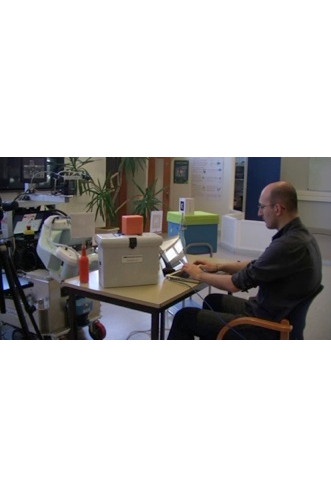
\includegraphics[width=0.2\textwidth]{reachex-1.png} }
%    \subfigure[] {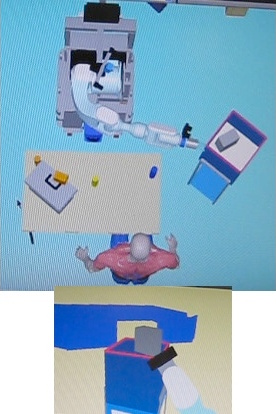
\includegraphics[width=0.2\textwidth]{reachex-2.jpg} }
%    \subfigure[] {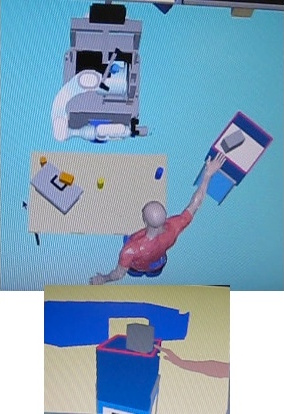
\includegraphics[width=0.2\textwidth]{reachex-3.jpg} }
%    \subfigure[] {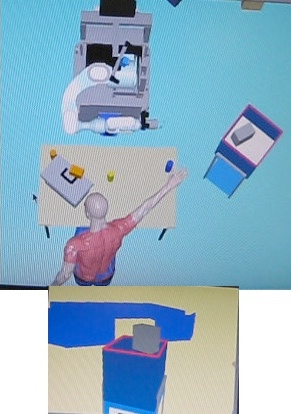
\includegraphics[width=0.2\textwidth]{reachex-4.jpg} }
%    \caption{An example illustrating the \textit{reachable} relation. The
%        relation is computed from the perspectives of both the robot and the
%        human. The computed posture at each step is illustrated with a global
%        view of the scene (top), and from a closest view (bottom). The robot
%        and its human partner are placed face to face (a).  The robot first
%        estimates if the small grey box is reachable to itself using an inverse
%        kinematic (IK) solver and collision checks to find a collision free
%        posture to reach the object (b). Next the robot switches to the human's
%        perspective to estimate if the same object is reachable to the human as
%        well (c).  In the last scene, the human moves towards his left, farther
%        from the object (d). The situation is then reevaluated. In this occasion
%        though, the reasoner cannot find a satisfactory posture for the human to
%    reach the box because he is too far from the target.  }
%
%\label{fig::reach-ex}
%\end{figure*}
%

\paragraph{Hypotheses on Objects States and Positions}

Occlusions, be they purposeful (when an agent hides an object behind or inside
another one) or not, commonly lead to difficulties in perceiving and tracking
objects in certain states. To mitigate this issue, {\sc Spark} also models the
possible symbolic states of objects (whether the object is on a furniture, in an
agent hand, in a container, etc.) with an associated probability distribution
based on the robot's perception of what has happened since the object was last
seen.  This probabilistic model of the environment is not currently integrated
with the knowledge base, and is instead directly queried by the execution
controllers when necessary.

\subsubsection{Primitive Action Recognition}

Monitoring human activity is needed by the execution controllers to track the
engagement of the human and the progress of his/her actions and also to synchtronize seamlessly
its own actions with the human actions. Full human action
and activity recognition is a task that requires knowledge and reasoning both on
high-level facts like goals, intentions and plans, as well as bottom-up data
from human and object motions. {\sc Spark} implements a set of simple temporal and
geometric heuristics on human hand trajectories and possible objects placements
to recognize simple atomic actions. Those primitive actions are assessed through
monitoring situations like ``an empty hand is close to an object on a table''
(precursor for a \emph{pick}), or ``a hand holding an object is over a
container'' (precursor for a \emph{throw}).  {\sc Spark} recognises a set of
such primitives. When combined with the other geometric computations and a predictive
plan of the human actions (see Section~\ref{hatp}), the execution controller can
track the fulfilment of the pre- and post-conditions of the predicted human
actions. As a result, the robot can monitor the engagement of the human and the
overall progress of the human-robot shared plan.

\subsubsection{Limitations}

In its current form, our situation assessment module makes two strong
assumptions: the objects are known in advance (hence, we can rely on proper 3D
CAD model for spatial reasoning) and the robot benefits of an almost perfect
perception, made possible by the use of fiducial markers.  Each object receives
a unique tag which enables us to accurately localize it in 3D and prevent
recognition ambiguities that would be then reflected in the knowledge base.
While {\sc Spark} algorithms themselves are ignorant of the input sources, and
would work equally well with a full object recognition stack, we are yet to
investigate this research area.

Additionally, temporal reasoning (essential for accurate action recognition for
instance) is not properly addressed in the current version of our system. Temporal reasoning is used
only locally, and does not allow for tracking of long sequences or global events.


%%%%%%%%%%%%%%%%%%%%%%%%%%%%%%%%%%%%%%%%%%%%%%%%%%%%%%%%%%%%%%%%%%%%%%%%%%%%%%%%
\subsection{Multi-Modal Communication}
\label{sect|com}

\subsubsection{Natural Language Grounding}

Natural language is a basic interaction modality that we use in our system both
as an input (processing of the human speech) and as an output (verbalization of the
robot intentions). Natural language processing is facilitated by our architecture
that processes information with semantics that are already close to a
human-level. This section presents the main features of our speech processor,
{\sc Dialogs}, that include semantic and multi-modal grounding, and interactive
disambiguation. Algorithmic and implementation details are provided
in~\cite{Lemaignan2011a}.

We acquire natural speech input from the human participants through a custom
Android-based interface. The interface relies on the Google speech recognition API for
speech-to-text and relays the textual transcript to the robot. The text is parsed into
a grammatical structure (\emph{Part of Speech} tagging), and the atoms of each
sentence are resolved with the help of the ontology to ground concepts like
objects (\ie when a user says ``pick up the can'', it resolves to which instance of
\emph{can} the user is referring to) and actions.  Figure~\ref{dialogs|ex} gives
an example of the processing of a simple, non-ambiguous command. The first
study (Section~\ref{moving-london}) walks through more complex examples.
Heuristics, like the presence of a question mark or the use of imperative mood,
are used to classify the sentences into questions, desires or statements.
{\sc Dialogs} processes these accordingly by answering questions or
updating the knowledge base.

\begin{figure}
    \centering
    \begin{tabular}{l}
        \emph{Initial human knowledge} \\
        \hline
        \stmt{book\_1 type Book} \\
        \stmt{human\_1 type Human} \\
        ~\\
        ~\\
        ~\\
    \end{tabular}
    \begin{tabular}{l}
        \emph{Input}\\

        \hline

        \concept{human\_1} says:\\
        ``Give me the book'' \\
        ~\\
        ~\\
        ~\\

    \end{tabular}
    \begin{tabular}{l}

        \emph{Generated query to ontology} \\
        \hline
        \concept{find(?obj type Book)} \\ 
        \hspace{0.2cm}$\Rightarrow$ \concept{?obj = book\_1} \\
        ~\\
        ~\\
        ~\\
    \end{tabular}
    \begin{tabular}{l}

        \emph{Newly created statements}\\
        \hline
        \stmt{human\_1 desires sit\_1} \\
         \stmt{sit\_1 type Give} \\
         \stmt{sit\_1 performedBy myself} \\
         \stmt{sit\_1 actsOnObject book\_01} \\
         \stmt{sit\_1 receivedBy human\_1} \\
    \end{tabular}

    \caption{Processing of a simple, non-ambiguous command, taken
        from~\cite{Lemaignan2011a}. Thematic roles ({\tt performedBy}, {\tt
        actsOnObject}, {\tt receivedBy}) are automatically extracted by 
    {\sc Dialogs} from the imperative sentence ``Give me the book.'' The 
    resulting statements (right column) are added to the knowledge base, and
    may eventually trigger an event in the execution controller (see
    Section~\ref{events}).}

    \label{dialogs|ex}
\end{figure}


The system supports quantification (``give me \{a | the | some | all | any |
$n$\} can''), thematic roles (action-specific predicates that qualify the
actions), interactive disambiguation (the robot asks questions when it needs
more information), and anaphora resolution (``give \emph{it} to me'') based on
dialogue history. It also supports knowledge extension by learning new semantic
structures. For instance, a sentence like ``learn that cats are animals'' is
converted into \stmt{Cat subClassOf Animal} and added to the knowledge base
after checking for possible contradictions with existing knowledge. {\sc
Dialogs} finally interprets common temporal and spatial adverbs (like
\emph{above} or \emph{tomorrow}) and translates simple expressions of internal
state  into \emph{experiences} (for instance, ``I'm tired'' is processed into
\stmt{human\_1 experiences state\_1, state\_1 hasFeature tired}, see also
Section~\ref{sect:desires}). A full account of the {\sc Dialogs} features and
the corresponding algorithms is available in~\cite{Lemaignan2011a}.

\subsubsection{Multi-Modality}

Because the components of our architecture rely on the same RDF formalism to
represent their outputs, the different communication modalities are presented in
a homogeneous way, as symbolic statements in the knowledge base. This applies
both to \emph{explicit} modalities (verbal communication, deictic gestures,
social gaze), and \emph{implicit} modalities (like the body position of the
human). The dialogue grounding process makes use of them at two distinct levels
to provide multi-modal concept grounding.

First, specific steps of the grounding process explicitly check for the presence
and value of certain facts. For instance, when several instances match a
category (the human says ``give me the bottle'' and the robot knows about three
bottles), the module may decide to discard some of the candidates based on their
\emph{visibility} for the speaker (implicit communication context taking into
account the human position). In this particular case, the heuristic is selected
by {\sc Dialogs} based on the quantifier preceding the class (``give me
\underline{the} bottle''). The first study (Section~\ref{moving-london})
illustrates the details of this process.

As another example, when the human says ``this'', the robot checks if the human
is currently pointing at an object. In that case, \emph{this} is replaced by the
object focused on. Otherwise, the robot performs anaphora resolution by looking
up in the dialogue history to find a previous concept that the user could refer
to.

Note that while the system benefits from complementary modalities, they are not
all required. The system can run with the verbal modality alone, at the cost of
a simpler interaction. For example, if the human says ``this'' without the robot
tracking what the human points at, no \stmt{human\_1 pointsAt ...} fact would
possibly be available in the knowledge base, and the robot falls back on the
anaphora resolution step alone.

The second level of integration of multi-modality is implicit. By continuously
computing symbolic properties from the geometric model, richer symbolic
descriptions are available to the system to verbalize or discriminate entities.
For instance, the robot may compute that one bottle is next to a glass, while
another one stands alone. These symbolic descriptions are transparently
re-used in a dialogue context to generate unambiguous references to discriminate
between similar objects: ``do you mean the bottle that is next to the glass?''.
The physical context of the interaction is used as an implicit communication
modality by {\sc Dialogs}. \cite{Ros2010b} provides a detailed account of our
approach toward interactive concept clarification and discrimination, along with the
related algorithms.

%%%%%%%%%%%%%%%%%%%%%%%%%%%%%%%%%%%%%%%%%%%%%%%%%%%%%%%%%%%%%%%%%%%%%%%%%%%%%%%%

\subsection{Human-Aware Task Planning}
\label{hatp}

Our execution controllers rely on symbolic task planning to convert long-term
desires into a succession of atomic actions. Our architecture uses the HATP
planner (\emph{Human Aware Task Planner})~\cite{Alili2008,
Alili2009,Lallement2014}.

The HATP planning framework extends the traditional Hierarchical Task
Network (HTN) planning domain representation and semantics by making them more
suitable to produce plans which involve humans and robots acting together
toward a joint goal. HATP is used by the robot to produce human-robot
\emph{shared plans}~\cite{Grosz1996,Clark1996,Kemp2007} which are then used to
anticipate human action, to suggest a course of action to humans, or even to ask
help from the human.

The HATP planning domain defines a set of methods describing how to
decompose a task and represents the procedural knowledge of the robot as well as
its knowledge about the actions that the human partner is able to achieve. It is
stored outside of the central knowledge base, using a specific formalism (see
the related discussion at the end of this section).

\subsubsection{Agents and Action Streams}

The originality of HATP resides in its ability to produce plans for the robot's
actions as well as for the other participants (humans or robots), that we
call \emph{shared plans}. 

HATP treats agents as ``first-class
entities'' in the domain representation language. It can therefore
distinguish between the different agents in the domain as well as
between agents and the other entities such as tables and chairs. This
enables a post-processing step that splits the final
solution (sequence of actions) into two (or more if there are several
humans) synchronised solution
streams, one for the robot and one for the human, so that the streams may be executed in
parallel and synchronised when necessary (Figure~\ref{plan_hatp1}).

This effectively enriches the interaction capabilities of the robot by providing
the system with what is in essence a prediction of the human behaviour. This
prediction is used by the robot execution controller to monitor the engagement
of the human partner during joint tasks.

The planner also generates synchronisation points between the agents. For
instance, in the plan depicted on Figure~\ref{plan_hatp1}, the human needs to
wait for the success of the robot's action {\tt PUTRV}. The robot monitors the
success of its own action (by checking for the fulfilment of the action
post-conditions; in this particular case \stmt{HUMAN sees BOTTLE} and
\stmt{HUMAN canReach BOTTLE}) to estimate what and when the human is likely to
perform his next action (here, \concept{TAKE(BOTTLE, TABLE)}). This, in turn,
allows the robot to monitor the human engagement and progress in the shared
plan.

We also use shared plans to verbalise the sequence of actions and to explain
the human partner how a task may be shared~\cite{warnier2012when}.

\begin{figure}[htbp]
    \centering
\resizebox{0.9\textwidth}{!}{%
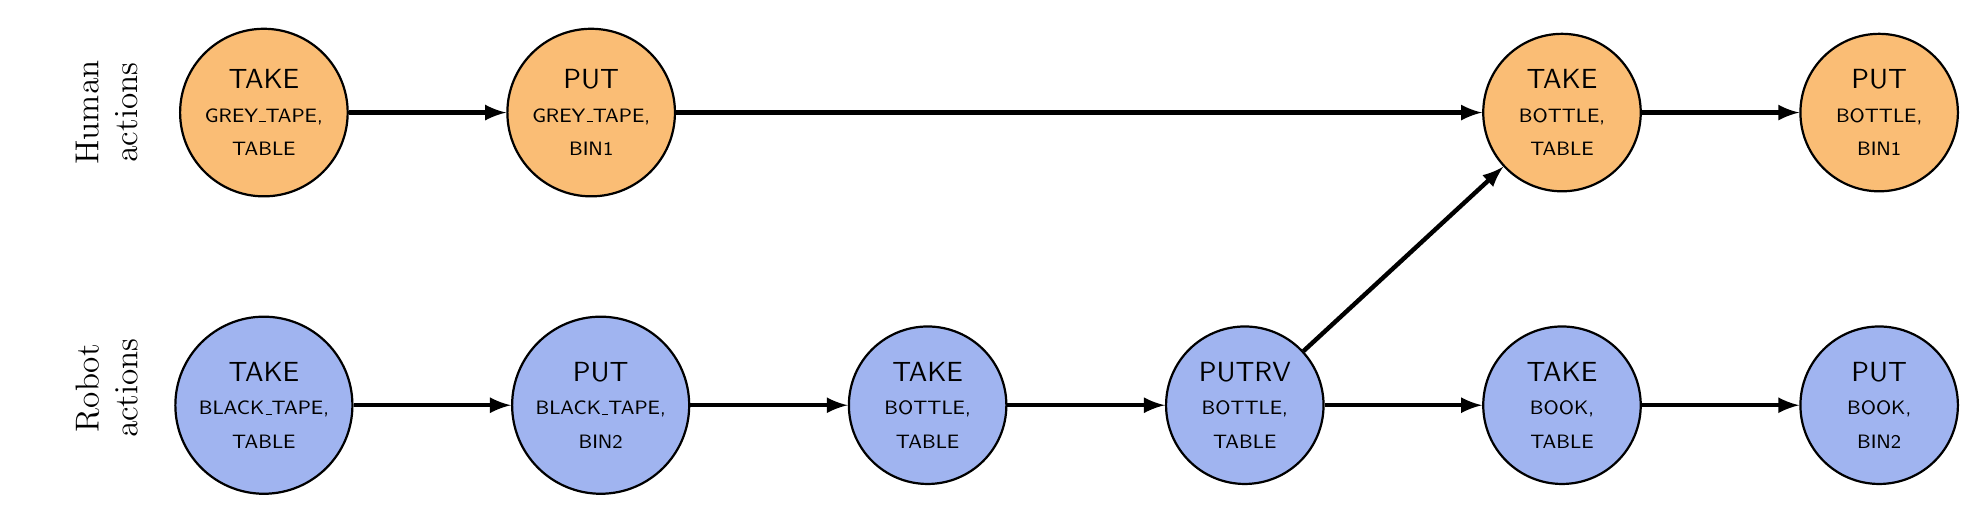
\begin{tikzpicture}[
    >=latex,
    robot/.style={fill=RoyalBlue!50},
    every edge/.style={<-, draw, ultra thick},
    every node/.style={ draw, 
                        thick,  
                        circle, 
                        font=\sf,
                        align=center,
                        node distance=2cm,
                        fill=BurntOrange!50, 
                        minimum size=2cm, 
                        inner sep=0.1cm}]

    \node[font=\rm\large, draw=none, fill=none, rotate=90] at (-2, 0) {Human\\actions};
    \node[font=\rm\large, draw=none, fill=none, rotate=90] at (-2, -3.5) {Robot\\actions};

    \node (h1) {\action{TAKE}{GREY\_TAPE}{TABLE}};
    \node[right=of h1] (h2) {\action{PUT}{GREY\_TAPE}{BIN1 }} edge (h1);

    \node[robot, below=1.5 of h1] (r1) {\action{TAKE}{BLACK\_TAPE}{TABLE }};
    \node[robot, right=of r1] (r2) {\action{PUT}{BLACK\_TAPE}{BIN2 }} edge (r1);
    \node[robot, right=of r2] (r3) {\action{TAKE}{BOTTLE}{TABLE }} edge (r2);
    \node[robot, right=of r3] (r4) {\action{PUTRV}{BOTTLE}{TABLE}} edge (r3);
    \node[robot, right=of r4] (r5) {\action{TAKE}{BOOK}{TABLE }} edge (r4);
    \node[robot, right=of r5] (r6) {\action{PUT}{BOOK}{BIN2 }} edge (r5);

    \node at (r5 |- h1) (h3) {\action{TAKE}{BOTTLE}{TABLE}} edge (h2) edge (r4);
    \node[right=of h3] (h4) {\action{PUT}{BOTTLE}{BIN1}} edge (h3);

\end{tikzpicture}
}

\caption{An example of plan produced by HATP for a task consisting in
    cooperatively moving objects into their associated bins. Two action streams
    are generated (human actions at the top, robot actions at the bottom, {\sf
    PUTRV} stands here for {\it Put it so it is both reachable and visible}).
    The arrow between the two streams represents a synchronization point.}

  \label{plan_hatp1}
\end{figure}

\subsubsection{Action Costs and Social Rules}

A cost and a duration function are associated to each action.  The duration
function provides a duration interval for the action achievement and is used, in
one hand, to schedule the different streams and, on the other hand, as an
additional cost function.

HATP includes mechanisms called \emph{social rules} to filter plans so as to
keep only those considered as suitable for human-robot interaction. The planner
allows for the specification of the following filtering criteria:

\emph{Wasted time}: avoids plans where the human spends a lot
of its time being idle,

\emph{Effort balancing}: avoids plans where efforts are
not fairly distributed among the agents taking part to the plan.  It is
indeed sometimes beneficial to balance efforts between the human and
the robot,

\emph{Simplicity}: avoids plans with too many interdependencies
between the actions of agents mentioned in the plan, as a problem with
executing just one of those actions could invalidate the entire
plan. Also intricate human-robot activity may cause discomfort since
the human will find himself repeatedly in a situation where his is
waiting for the robot to act,

\emph{Undesirable sequences}: avoids plans that violate specific user-defined
sequences (for instance sequences which can be misinterpreted by the human).

Combining the above criteria, we typically yield shared plans with desirable
interaction features like the human still being engaged in a number of tasks
while its overall level of required efforts remains low, or avoiding having the
human to wait for the robot (by essentially preventing the action streams from
having too many causal links between them).

Figure~\ref{plan_hatp2} illustrates such a socially-optimised plan where the
\emph{no wasted time} social rule is applied: compared to the plan depicted in
Figure~\ref{plan_hatp1}, the robot first moves the bottle so that the human can
immediately take it and put it into the bin, thus removing the human idle time.
The resulting shared plan is considered better than the one depicted on
Figure~\ref{plan_hatp1} according to a global evaluation of the costs and rules.

In the current implementation, the social rules are effectively
implemented by looking through all the plans produced and filtering
out the ones that do not meet the desired requirements. In the
future we intend to study algorithms that do such filtering online,
rather than after initial solutions are found.

\begin{figure}[htbp]
  \centering
\resizebox{0.9\textwidth}{!}{%
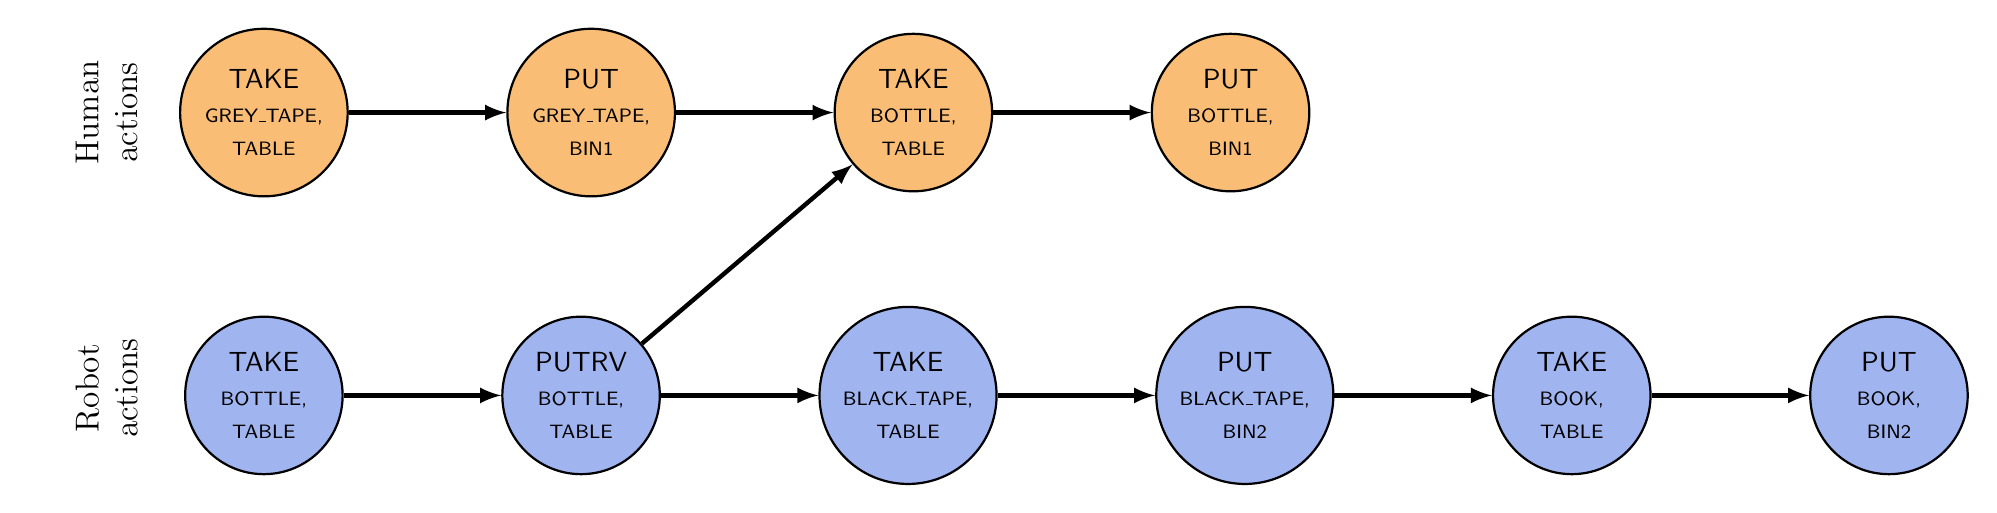
\begin{tikzpicture}[
    >=latex,
    robot/.style={fill=RoyalBlue!50},
    every edge/.style={<-, draw, ultra thick},
    every node/.style={ draw, 
                        thick,  
                        circle, 
                        font=\sf,
                        align=center,
                        node distance=2cm,
                        fill=BurntOrange!50, 
                        minimum size=2cm, 
                        inner sep=0.1cm}]

    \node[font=\rm\large, draw=none, fill=none, rotate=90] at (-2, 0) {Human\\actions};
    \node[font=\rm\large, draw=none, fill=none, rotate=90] at (-2, -3.5) {Robot\\actions};


    \node (h1) {\action{TAKE}{GREY\_TAPE}{TABLE}};
    \node[right=of h1] (h2) {\action{PUT}{GREY\_TAPE}{BIN1 }} edge (h1);

    \node[robot, below=1.5 of h1] (r3) {\action{TAKE}{BOTTLE}{TABLE }};
    \node[robot, right=of r3] (r4) {\action{PUTRV}{BOTTLE}{TABLE}} edge (r3);
    \node[robot, right=of r4] (r1) {\action{TAKE}{BLACK\_TAPE}{TABLE }} edge (r4);
    \node[robot, right=of r1] (r2) {\action{PUT}{BLACK\_TAPE}{BIN2 }} edge (r1);
    \node[robot, right=of r2] (r5) {\action{TAKE}{BOOK}{TABLE }} edge (r2);
    \node[robot, right=of r5] (r6) {\action{PUT}{BOOK}{BIN2 }} edge (r5);

    \node[right=of h2] (h3) {\action{TAKE}{BOTTLE}{TABLE}} edge (h2) edge (r4);
    \node[right=of h3] (h4) {\action{PUT}{BOTTLE}{BIN1}} edge (h3);

\end{tikzpicture}
}

    \caption{An alternative plan for the task presented in
    Figure~\ref{plan_hatp1} where the \emph{no wasted time} social rule is used to optimise the
total duration of the task. }

  \label{plan_hatp2}
\end{figure}

%\subsubsection{Commitment Levels}
%
%By tuning its costs and adapting its social rules, HATP can be used to compute
%various alternative plans. These plans can be categorised into several levels of
%cooperation
%
%\begin{itemize}
%\item helping the human to achieve his goal by acting for him
%\item sharing concrete resources by handing some objects
%\item collaboration of the robot and the human by coordinating their
%  actions towards a human-robot joint goal.
%\end{itemize}
%

As HATP is a generic symbolic task planner and do not enforce any abstraction
level for the planning domain, we were able to design a domain built from
top-level tasks whose semantics are close to the one used in the human-robot
dialogue: the planner domain effectively contains concepts like \texttt{give},
\texttt{table}, \texttt{is on}. This leads to an effective mapping between the
knowledge extracted from the situation assessment or the dialogue, and the
planner.

Also, we would like to mention that, after some research we have decided against
representing the planning domain (\ie, the set of tasks with their pre- and
post-conditions) in the knowledge base itself due to expressiveness issues (see
appendix B of~\cite{Lemaignan2012a} for a detailed discussion). This effectively
leads to independent declarative and procedural knowledge stores.

%%%%%%%%%%%%%%%%%%%%%%%%%%%%%%%%%%%%%%%%%%%%%%%%%%%%%%%%%%%%%%%%%%%%%%%%%%%%%%%%
\subsection{Robot Execution Control}
\label{sect|ctrl}

While parts of the architecture ({\sc Spark}, {\sc Oro}) have been deployed with
external execution controllers (like {\sc Cram}~\cite{Beetz2010} or the BERT
platform~\cite{Lallee2010b}, as reported in~\cite{Lemaignan2010}), we have also
developed dedicated robot controllers which integrate the whole stack introduced
in Figure~\ref{fig|archi}. {\sc Shary}~\cite{clodic2008shary} is the main one,
written in the \emph{Procedural Reasoning System} language~\cite{Ingrand1996}.
We have also developed the Python-based {\sc pyRobots}~\cite{lemaignan2015pyrobots} that
provides a large set of high-level actions and an event-based architecture well
suited for prototyping. They both rely on extensive integration with the knowledge
base, that serves as the primary source of semantics for the decision making process.

One of the main roles of {\sc Shary} is to control the production and execution
of shared plans. This means essentially context-based refinement and robot
actions execution, as well as monitoring of those achieved by its human
partner. One of the key design goal is to build such abilities in a generic
way, and to provide several levels of parametrisation allowing to adapt to
various environments, and various levels of involvement of the robot ranging
from teammate behaviour to assistant or proactive helper. Based on this,
the robot controller invokes the adequate human-aware planners and react to
events triggered by the {\sc Oro} knowledge base (as described below).

{\sc Shary}'s originality, as an execution control system, lies in its ability
to take into account not only the task achievement but also the communication
and monitoring needed to support interactive task
achievement~\cite{Rich1997,Sidner2005} in a flexible manner. {\sc Shary} allows
to bind action execution to \emph{communication policies} in order to produce
signals towards the human and to react to human actions. The
\emph{communication act} is the central concept in this formalism. It
represents an information exchange between the two agents and plays the role of
a transition condition. This exchange can be realised through dialogue, by an
expressive motion or a combination of the two. It enables each agent to
communicate their beliefs about the task to be achieved, in order to share
mutual knowledge and to synchronise their activities.  This is done through
real-time task-based situation assessment achieved by the combination of {\sc
Shary} monitoring processes and {\sc Oro} inference
mechanisms~\cite{fiore2014}. \fixme{Rachid, reviewer 2 asks for more details
about this process -> M. Fiore work?}



\subsubsection{Event-Driven Control}
\label{events}

The {\sc Oro} server supports two paradigms to access its content: RPC-style
queries (based on the standard SPARQL language) or events. A module can
subscribe to an event by passing through an event pattern (in its simplest
form, a partial statement like \stmt{? type Book}) and a callback.  Each
time a new instance of a book appears in the knowledge base, the callback is
triggered.

This allows us to write reactive robot controllers with a high level of
expressiveness: for instance, by subscribing to the event \stmt{human1 desires
?action, ?action type Give, ?action actsOnObject ?obj, ?obj type Book}, we could
trigger a behaviour when the human expresses (through dialogue, gestures...)
that he wants the robot to give her a book.

The robot controller designer does not need to directly care about how this
\emph{desire} is produced (this is delegated to perception modules), he can
focus on the semantic of the desire.

Note also that we take advantage of the reasoning capabilities of the system:
for example, the type of the object (\stmt{?obj type Toy}) may not be
explicitly asserted, but inferred by the reasoner based on other assertions.

\subsubsection{Desires and Experiences}
\label{sect:desires}

We divide the interaction situations perceived from the situation assessment and
the communication components into two categories: \emph{desires} (related to
\emph{performative acts} in Austin's classification of speech
acts~\cite{Austin1962}) and \emph{experiences}.

\emph{Desires} are typically human commands (``Give me that book''). The nature of
the desired action (to pick, to give, to look, to bring, to show...), along with the action
parametrization (thematic roles) are extracted from the knowledge base, and
either passed to the task planner or executed if the procedure is directly
available.

\emph{Experiences}, on the other hand, comprise of emotions, states and
questions (when asking a question, we consider the human to be in an
\emph{interrogative state}). When the knowledge base states that an agent
\emph{experiences} a particular emotion or state, the execution controller may
decide to handle it, typically by trying to answer the question or using the
emotional or physical state as a parameter for subsequent actions. As an
example, when the speaker says ``I feel tired'', we change the motion planner
parametrization to lower the effort the human needs to provide for the following
joint manipulation tasks.\footnote{Note that this specific example has been
implemented as a proof-of-concept. A broader framework that would support
action alteration based on the user's experienced states remains to be investigated.}

\subsubsection{Action Execution and Monitoring}\label{sec:action}

Like most robotic architectures, actions are split into \emph{atomic actions}
that are combined into \emph{tasks}. Tasks are created either statically or dynamically.
The {\sc pyRobots} controller, for instance, statically combines the actions listed in
table~\ref{table|pyrobots_actions} to implement the high-level tasks it exposes: {\tt
lookAt}, {\tt moveTo}, {\tt getFromHuman}, {\tt showObject}, {\tt giveObject},
{\tt pickObject}, {\tt bringObject}, {\tt putObject}, {\tt hideObject}.
Our other controller, {\sc Shary}, relies on the symbolic task planner to
dynamically generate, at run-time, suitable sequence of atomic actions.

\begin{table}[ht!]
\begin{center}
\begin{tabular}{p{0.8\columnwidth}}
\hline
    {\bf Manipulation} \\
     {\tt attachobject}, {\tt basicgive}, {\tt basictake}, {\tt close\_gripper}, {\tt configure\_grippers}, {\tt grab\_gripper}, {\tt handover}, {\tt hide}, {\tt open\_gripper}, {\tt pick}, {\tt put}, {\tt put\_accessible}, {\tt release\_gripper}, {\tt show}, {\tt take} \\
\hline
    {\bf Gaze control} \\
     {\tt glance\_to}, {\tt look\_at}, {\tt sweep}, {\tt switch\_active\_stereo\_pair}, {\tt track}, {\tt cancel\_track} \\
\hline
    {\bf Navigation} \\
     {\tt carry}, {\tt follow}, {\tt cancel\_follow}, {\tt goto}, {\tt moveclose}, {\tt waypoints} \\
\hline
    {\bf Local navigation} \\
     {\tt dock}, {\tt rotate}, {\tt translate} \\
\hline
    {\bf Posture configuration} \\
     {\tt extractpose}, {\tt idle}, {\tt manipose}, {\tt movearm}, {\tt rest}, {\tt setpose}, {\tt settorso}, {\tt tuckedpose} \\
\hline
\end{tabular}
\end{center}
\caption{Main {\sc pyRobots} actions, sorted by categories. These
actions are combined at run-time into higher-level \emph{tasks}.}

\label{table|pyrobots_actions}
\end{table}

The symbolic manipulation and navigation actions listed in
Table~\ref{table|pyrobots_actions} are eventually executed by the execution
controller with the help of a dedicated 3D motion planner (called {\sc Mhp},
Figure~\ref{fig|archi}): robot placement and end-effectors trajectories are
computed on-line to allow object manipulation that take into account task
specific constraints and human postures, abilities and preferences.  We kindly
refer the interested reader to~\cite{Sisbot2008, Mainprice2011, Pandey2011} for
details of these techniques.


%\paragraph{Action Execution and Monitoring Robot Controller}
%Based on context and on the shared plan produced by HATP for a given goal,
%the robot controller decides to execute an action or to ask its human
%partner to do it.  Actions feasibility by the human or the robot are
%regularly reconsidered based on the reachability / visibility
%computation mechanisms.
%
%Robot action execution is based on simple automatons  that translate
%symbolic planning atomic actions into sequences of planned arm motions
%and gripper commands to execute according to current state
%of the 3-tuple (gripper, object, furniture). We have three states
%according to whether the object is in gripper and if it is in gripper
%whether it is on furniture.  These states are directly obtained from
%the updated symbolic state of the world in the ontology.
%
%For plan action monitoring, primitive actions recognition is used. A primitive
%action detection is interpreted as action success if it is the expected one and
%failure otherwise. The robot also reacts to the absence of activity.
%


%%%%%%%%%%%%%%%%%%%%%%%%%%%%%%%%%%%%%%%%%%%%%%%%%%%%%%%%%%%%%%%%%%%%%%%%%%%%%%%%
%%%%%%%%%%%%%%%%%%%%%%%%%%%%%%%%%%%%%%%%%%%%%%%%%%%%%%%%%%%%%%%%%%%%%%%%%%%%%%%%
%%%%%%%%%%%%%%%%%%%%%%%%%%%%%%%%%%%%%%%%%%%%%%%%%%%%%%%%%%%%%%%%%%%%%%%%%%%%%%%%

\section{Support Studies}
\label{sec:expe}

Our architecture has been deployed and tested in a number of studies on
several robotic platforms. Table~\ref{table|experiments} lists the most
significant ones, with their main focuses and reference publications.

\begin{table*}
\begin{center}

\begin{tabular}{lll}
 \bf{Study} & Focus & Reference \\
\hline
{\it Point \& Learn} (2010) & Interactive knowledge acquisition & \cite{Lemaignan2010} \\
{\it Spy Game} (2010) & Interactive object discrimination & \cite{Ros2010b} \\
{\it Interactive Grounding I} (2011) & Multi-modal interaction, perspective taking & \cite{lemaignan2011what} \\
{\it Roboscopie} (2011) & Human-Robot theatre performance & \cite{lemaignan2012roboscopie} \\
{\it Cleaning the table} (2011) & Complete architecture integration & \cite{Alami2011} \\
{\it I'm in your shoes} (2012) & False beliefs & \cite{warnier2012when} \\
{\it Give me this} (2012) & Natural joint object manipulation & \cite{gharbi2013natural} \\
{\it Interactive Grounding II} (2012) & Multi-modal interaction, perspective taking & \cite{lemaignan2013talking} \\
\hline

\end{tabular}
\end{center}
\caption{Main studies conducted with our cognitive architecture.}
\label{table|experiments}
\end{table*}

We present here elements of two of them in order to illustrate in a practical way
different aspects of the architecture.  The first one is focused on knowledge
representation and verbal interaction: the human asks for help to find and pack
objects ({\it Interactive Grounding I} in Table~\ref{table|experiments}). The
second one ({\it Cleaning the table}) involves the {\sc Shary} execution
controller and the HATP symbolic task planner. In this scenario, the human and
the robot try to cooperatively remove objects from a table, and behaviours and
motions are fully planned and then executed.

\subsection{Interactive Grounding}
\label{moving-london}

This first study is based on a ``home move'' backstory: two users are moving
their belongings to a different home, and need the help of a robot to pack.
\emph{Jido}, a single-arm mobile manipulator, is observing while they carry
over boxes (Figure~\ref{fig|vpt}), and answers questions pertaining to the
location of specific objects.  This study focuses on multi-modal, interactive
grounding only, and the robot does not actually perform any action besides
verbal interaction and simple head movements.

Objects are perceived solely through 2D fiducial markers sticked on them, and humans are
tracked through motion capture. The robot knowledge base is initialised with
the {\sc Oro} commonsense ontology.  We next describe two
situations where we can follow the internal robot's reasoning and the
interaction with the user.

\paragraph{Implicit Disambiguation Through Visual Perspective Taking}

\begin{figure}[!ht]
  \centering
  \subfigure [Interactive grounding in a cluttered environment.]{
  \label{fig|vpt}
  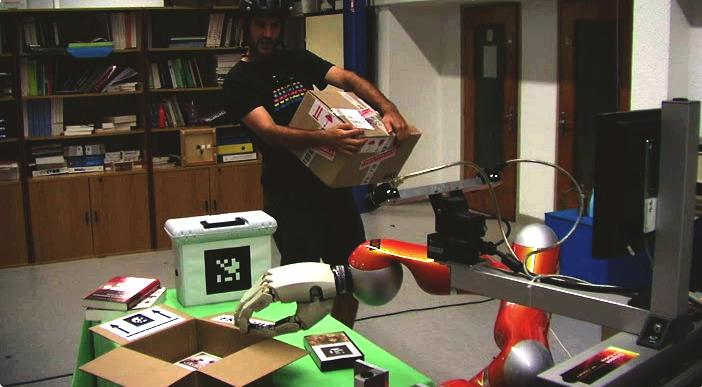
\includegraphics[width=0.48\linewidth]{pt.jpg}
}%
\subfigure [Disambiguation through pointing.]{
  \label{fig|pointing}
  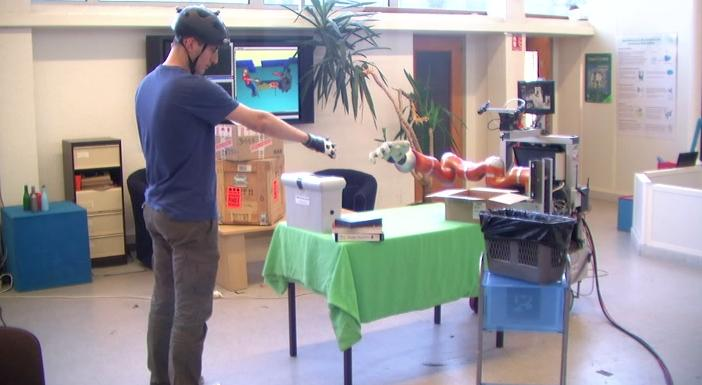
\includegraphics[width=0.48\linewidth]{inTheBox2.jpg}
}
\end{figure}


User A enters the room while carrying a large box (Figure~\ref{fig|vpt}). He
approaches the table and asks Jido to hand him the video tape: ``Jido, can
you give me the video tape''. The \textsc{Dialogs} module processes this
sentence, and queries the ontology to
identify the object the human is referring to: \concept{find(?obj type
VideoTape)}. 

Two video tapes are visible to the robot: one on the table, and another one
inside the cardboard box. Thus, the knowledge base returns both: 
\concept{?obj = [BLACK\_TAPE, WHITE\_TAPE]}. 

However, only one is visible for User A (the one on the table). Although there is
an ambiguity from the robot's perspective, the human referred to the tape using
the definite article \emph{the}: this is interpreted by the natural language
processor as the human referring to a precise object, in that case, the visible
one.\footnote{Other heuristics are available to the {\sc Dialogs} module: for
instance, if a tape had been recently mentioned in the dialogue, this instance
would have been selected instead as the referent.}

%Since only one object remains (\ie the referent that \concept{VideoTape} stands
%for is not ambiguous any more), the robot infers that the human refers to it and
%eventually execute the command, \ie give it to the human. Alternatively, the
%robot first asks the human for confirmation (``was \concept{BLACK\_TAPE} the
%object you had in mind?'') before proceeding with the action.
%Table~\ref{table|ptbeliefs} lists the robot's beliefs about itself and its human
%partner involved in this situation.
%
%\begin{table}[ht!]
%\begin{center}
%    \subfigure{
%\begin{tabular}{l}
%\hline
%Robot's beliefs about itself (\emph{robot's model}):\\
%\hline
%  \hspace{0.7cm}\stmt{BLACK\_TAPE type VideoTape}\\
%  \hspace{0.7cm}\stmt{BLACK\_TAPE isOn table}\\
%  \hspace{0.7cm}\stmt{BLACK\_TAPE isVisible true}\\
%  \hspace{0.7cm}\stmt{WHITE\_TAPE type VideoTape}\\
%  \hspace{0.7cm}\stmt{WHITE\_TAPE isIn CARDBOARD\_BOX}\\
%  \hspace{0.7cm}\stmt{WHITE\_TAPE isVisible true}\\
%\hline
%\end{tabular}
%}\hspace{1em}%
%    \subfigure{
%\begin{tabular}{l}
%\hline
%Robot's beliefs about User A (\emph{User A's model}):\\
%\hline
%  \hspace{0.7cm}\stmt{BLACK\_TAPE type VideoTape}\\
%  \hspace{0.7cm}\stmt{BLACK\_TAPE isOn table}\\
%  \hspace{0.7cm}\stmt{BLACK\_TAPE isVisible true}\\
%  \hspace{0.7cm}\stmt{WHITE\_TAPE type VideoTape}\\
%  \hspace{0.7cm}\stmt{WHITE\_TAPE isIn CARDBOARD\_BOX}\\
%  \hspace{0.7cm}\stmt{WHITE\_TAPE isVisible false}\\
% \hline
%\end{tabular}
%}
%\end{center}
%\caption{Robot's beliefs about itself and its human partner.}
%\label{table|ptbeliefs}
%\end{table}
%
\paragraph{Explicit Disambiguation Through Verbal Interaction and Gestures}

In this second situation, User B enters the living room without knowing where
User A had placed the video tapes (Figure~\ref{fig|pointing}). So he first asks
Jido: ``What's in the box?''. The robot first need to ground the word ``box''.
Similar to the previous situation, two boxes are visible: \concept{find(?obj
type Box)} $\Rightarrow$ \concept{?obj = [CARDBOARD\_BOX, TOOLBOX]}

However both are visible to the human and the previous ambiguity resolution
procedure can not be applied. The robot generates a question (using the
\emph{Discrimination} algorithm, Section~\ref{reasoning})
and asks User B which box he is referring to by verbalizing the following question: ``Which box, the toolbox or the
cardboard box?'' User B can answer the question, but he instead decides to point
at it: ``This box'' (Figure~\ref{fig|pointing}). {\sc Spark} identifies the {\tt
CARDBOARD\_BOX} as being pointed at, as well as looked at, by the human and updates the
ontology with this new information. The reasonner applies a rule available in the common-sense
ontology \stmt{pointsAt(?ag, ?obj) $\land$ looksAt(?ag, ?obj) $\to$
focusesOn(?ag, ?obj)}. The \textsc{Dialogs} module merges both
sources of information, verbal (``this'') and deictic, by issuing a specific
query to the knowledge base that eventually lifts the ambiguity:

\begin{center} 
    \begin{tabular}{l} 
        \concept{find(?obj type Box; USER\_B focusesOn ?obj)}\\ 
        \hspace{0.7cm}$\Rightarrow$ {\tt ?obj = [CARDBOARD\_BOX]}
    \end{tabular} 
\end{center}

Finally, \textsc{Dialogs} queries the ontology about the content of the box and
the question can be answered: ``Wall-E'' (the label of the object is statically
asserted in the ontology).

%\begin{center}
%\stmt{?obj isIn CARDBOARD\_BOX}\\
%\hspace{0.7cm}$\Rightarrow$ \concept{?obj = WHITE\_TAPE}\\
%\end{center}

At this point User B wants to know where is the other tape: ``And where is the
other tape?''. \textsc{Dialogs} processes this sentence using the
\concept{differentFrom} OWL predicate:

\begin{center}
\begin{tabular}{l}
\stmt{?obj type VideoTape}\\
\stmt{?obj differentFrom WHITE\_TAPE}\\
\hspace{0.7cm}$\Rightarrow$ \concept{?obj = [BLACK\_TAPE]}
\end{tabular}
\end{center}

Since there is only one possible ``other'' videotape, no specific
disambiguation is required. The referent is uniquely identified and {\sc
Dialogs} can then query for its location. The robot finally verbalises the
result \stmt{BLACK\_TAPE isOn table, BLACK\_TAPE isNextTo TOOLBOX} into ``The
other tape is on the table and next to the toolbox.''

\subsection{\emph{Cleaning the table} Study}
\label{sec:cleantable}

\begin{figure}[ht!]
    \centering
    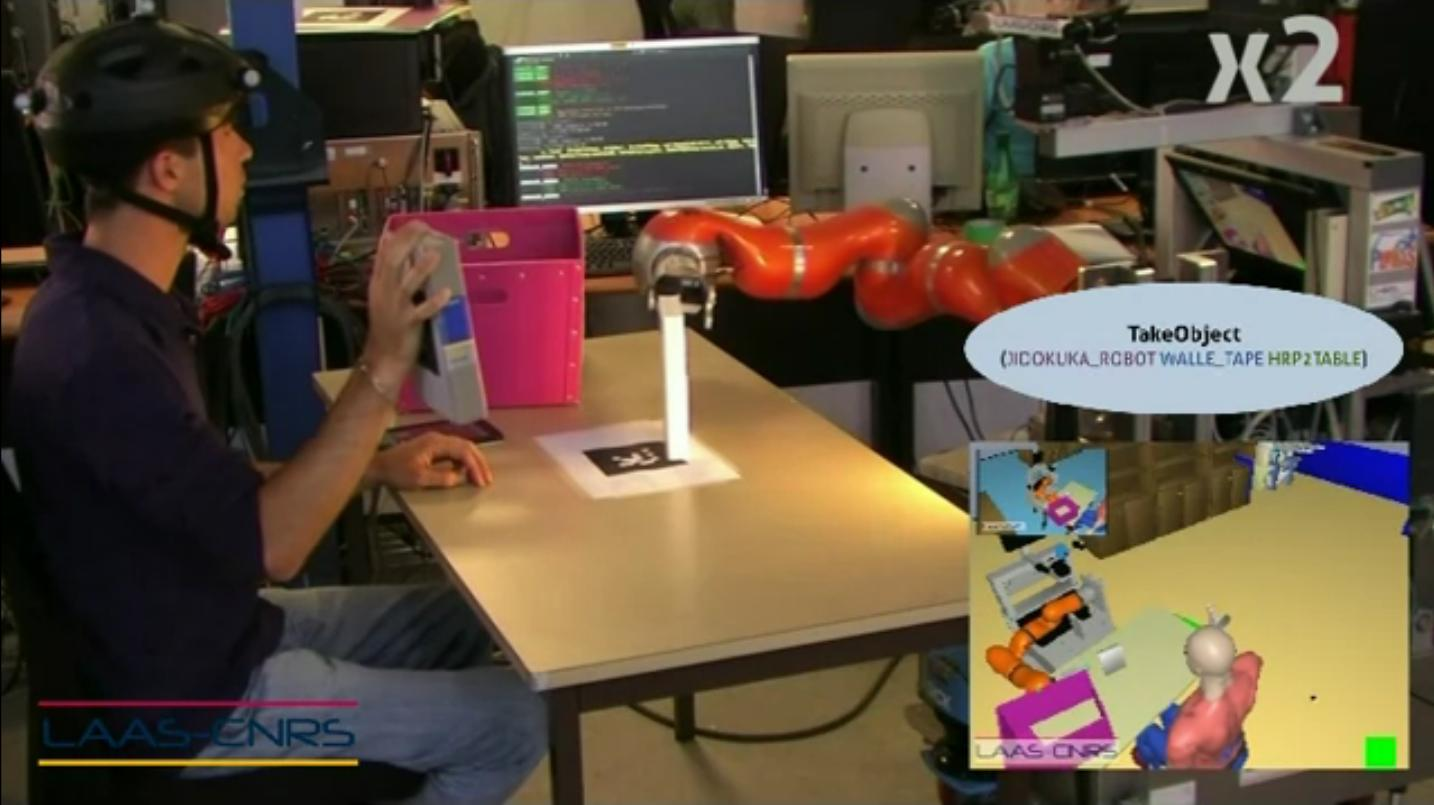
\includegraphics[width=0.6\columnwidth]{cleantable.jpg}

    \caption{The face-to-face setup of the \emph{Clean the Table} study. The
    physical situation, the {\sc Spark} model, and the current step of the plan
    are visible on the picture.}

    \label{fig|cleantable-video}
\end{figure}

This second study demonstrates a richer decision-making process where the {\sc
Oro} server is used in conjunction with the HATP symbolic task planner and the
{\sc Shary} execution controller to produce and execute a shared plan. The task
consists in cooperatively cleaning a table by moving objects into their target
bins (Figure~\ref{fig|cleantable-video}).

%In this scenario (Figure~\ref{fig|cleantable-video}), a human and a robot
%cooperate to remove objects from a table. The robot produces symbolic plans for
%both itself and the human (Figure~\ref{plan-etat2})
%that allow the robot to (verbally) share the task with the human (like ``I take
%the green box and I put it in the trashbin, you take the black video tape and
%you throw it in the trashbin''). Plans are created based on perceived
%visibility and reachability of the objects, and the robot also monitors the
%human activities to track the advancement of the whole plan.

%
%\begin{figure*}[thpb]
%  \centering
%\resizebox{0.9\textwidth}{!}{%
%\begin{tikzpicture}[
%    >=latex,
%    robot/.style={fill=RoyalBlue!50},
%    every edge/.style={<-, draw, ultra thick},
%    every node/.style={ draw, 
%                        thick,  
%                        circle, 
%                        font=\sf,
%                        align=center,
%                        node distance=2cm,
%                        fill=BurntOrange!50, 
%                        minimum size=2cm, 
%                        inner sep=0.1cm}]
%
%    \node[font=\rm\large, draw=none, fill=none, rotate=90] at (-2, 0) {Human\\actions};
%    \node[font=\rm\large, draw=none, fill=none, rotate=90] at (-2, -3.5) {Robot\\actions};
%
%
%    \node (h1) {\action{TAKE}{WALLE\_TAPE}{TABLE}};
%    \node[right=of h1] (h2) {\action{THROW}{WALLE\_TAPE}{TRASH\_1 }} edge (h1);
%
%    \node[robot, below=1.5 of h1] (r1) {\action{TAKE}{GREY\_TAPE}{TABLE }};
%    \node[robot, right=of r1] (r2) {\action{PUTRV}{GREY\_TAPE}{TABLE}} edge (r1);
%    \node[robot, right=of r2] (r3) {\action{TAKE}{LOTR\_TAPE}{TABLE }} edge (r2);
%    \node[robot, right=of r3] (r4) {\action{PUTRV}{LOTR\_TAPE}{TABLE }} edge (r3);
%
%    \node[right=of h2] (h3) {\action{TAKE}{GREY\_TAPE}{TABLE}} edge (h2) edge (r2);
%    \node[right=of h3] (h4) {\action{THROW}{GREY\_TAPE}{TRASH\_1}} edge (h3);
%    \node[right=of h4] (h5) {\action{TAKE}{LOTR\_TAPE}{TABLE}} edge (h4) edge (r4);
%    \node[right=of h5] (h6) {\action{THROW}{LOTR\_TAPE}{TRASH\_1}} edge (h5);
%
%
%\end{tikzpicture}
%}
%
%  \caption {A plan produced by HATP to execute the high-level order ``clean the
%  table''. Two streams of actions are generated: for the human (top) and for the
%  robot (bottom). Synchronization points ensure the coordination.}
%
%  \label{plan-etat2}
%\end{figure*}
%

Figure~\ref{fig|cleantable-timeline} walks through a simplifed version of the whole
task. It depicts a run with a single tape on a table. The tape is
reachable by the robot only, while the bin (where the objects are supposed to be
eventually moved to) is reachable by the human only: the robot needs to come up
with a shared plan that involves a joint action.

The goal is first received by the execution controller (after processing of the
user request by the {\sc Dialogs} module, not shown on the figure). At $t_1$ on
Figure~\ref{fig|cleantable-timeline}, the tape is computed by the robot as being
reachable by the robot only (columns \emph{Perception} and \emph{Knowledge}),
and the execution controller invokes the task planner, which produces a joint
plan (column \emph{Plan}) to move the tape so that the human can pick it and
drop it into the bin.

The first task (\concept{TAKE(GREY\_TAPE, TABLE)}) is instantiated by checking
that the task pre-conditions hold (in particular, \stmt{GREY\_TAPE isOn TABLE}
must be true), and calling the 3D motion planner (column \emph{Actions},
left). The motion planner returns two atomic actions ({\tt PICK\_GOTO} followed
by {\tt TAKE\_TO\_FREE}) that the controller executes (by first reaching for
the object, grasping it and bringing it back to a free position).  The robot's
perception monitors the evolution of the scene until the task's post-conditions
are verified (at $t_2$, by satisfying the statement \stmt{ROBOT hasInHand
TAPE}), and the next task is then started (placing the tape so that it becomes
reachable by the human).

At $t_3$, the tape is now reachable by the human, and the next tasks (taking the
tape and placing it in the bin) have to be performed by the human: the robot
instructs the user to do so (verbal interaction not pictured on the figure) and
monitors the actions of the human to detect when the tasks' post-conditions are
satisfied (column \emph{Actions}, right). When these post-conditions are
fulfilled, the goal is considered to be completed.

This simple example illustrates how the symbolic facts are produced from the
situation assessment, and, in parallel, used by the execution controller to
assess the overall progress of the plan.

\begin{figure*}[thpb]
  \centering

\renewcommand{\stmt}[1]{{\footnotesize \tt  #1}}
\resizebox{\textwidth}{!}{%
\begin{tikzpicture}[
        >=latex,
        box/.style={draw,rectangle, dotted, minimum width=#1, minimum height=3.8cm},
        box/.default={4.5cm},
        every edge/.style={draw, ultra thick, ->},
        every node/.style={align=center},
        robot/.style={fill=RoyalBlue!50},
        plan/.style={draw,
                     thick,  
                     circle, 
                     font=\sf,
                     align=center,
                     fill=BurntOrange!50, 
                     minimum size=1cm, 
                     inner sep=0.1cm}]


        \coordinate (figbottom) at (-0.5, -28.5);


        \fill[gray!10!white] (4.6,.5) rectangle (figbottom);

        \path (-0.5,0) edge (figbottom) node[sloped, above left, rotate=90] {\large\bf time};

        \node at (2,0) (percept) {\bf Perception};
            \node[below=0.5 of percept.south west, anchor=mid] {camera};
            \node[below=0.5 of percept.south east, anchor=mid] {3D model};

        \node[right=4 of percept, minimum width=2.5cm] (kb) {\bf Knowledge};
            \node[below=0.5 of kb.south west, anchor=mid east] (kbr) {robot};
            \node[below=0.5 of kb.south east, anchor=mid west] (kbh) {human};
            \draw[dotted] (kbr) to (figbottom -| kbr);
            \draw[dotted] (kbh) to (figbottom -| kbh);

        \fill[gray!10!white] (12,.5) rectangle (17,-28.5);
        \node[right=4.5 of kb] (plan) {\bf Plan};
            \node[below=0.5 of plan.south west, anchor=mid east] (probot) {robot};
            \node[below=0.5 of plan.south east, anchor=mid west] (phuman) {human};
            \draw[dotted] (probot) to (figbottom -| probot);
            \draw[dotted] (phuman) to (figbottom -| phuman);

        \node[right=5 of plan] (action) {\bf Actions};
            \node[below=0.5 of action.south west, anchor=mid east] (arobot) {robot};
            \node[below=0.5 of action.south east, anchor=west] (ahuman) {human\\(monitoring)};
            \draw[dotted] (arobot) to (figbottom -| arobot);
            \draw[dotted] (ahuman) to (figbottom -| ahuman);

        \draw[dashed] (-0.6,-1.2) --(24, -1.2);

        \node[anchor=east] at (-0.5, -3) (t1) {\Large $t_1$};
        \node[anchor=east, below=6 of t1] (t2) {\Large $t_2$};
        \node[anchor=east, below=6 of t2] (t3) {\Large $t_3$};
        \node[anchor=east, below=4 of t3] (t4) {\Large $t_4$};
        \node[anchor=east, below=5 of t4] (t5) {\Large $t_5$};

        %%%%%%%%%%%%%%%%%%%%%%%%%%%%%%%%%%%%%%%%%%%%%%%%%%%%%%%%%%%%%%%%%%%%%%%%%%%%%%%%%%%%%%%%%%%%
        %%% PERCEPTIONS
        %%%%%%%%%%%%%%%%%%%%%%%%%%%%%%%%%%%%%%%%%%%%%%%%%%%%%%%%%%%%%%%%%%%%%%%%%%%%%%%%%%%%%%%%%%%%

        \node at (t1 -| percept) (cam1) {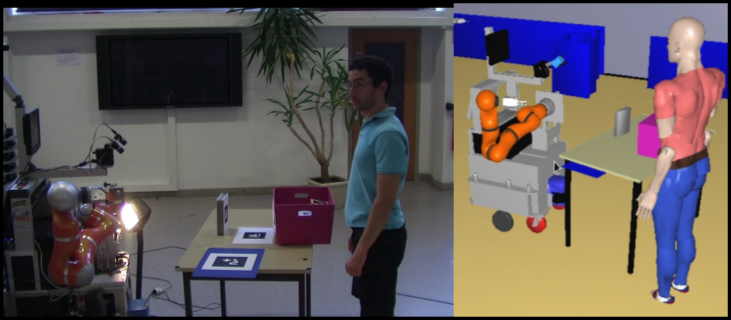
\includegraphics[height=2cm]{manip_run_cam1.png}};
        \node at (t2 -| percept) (cam2) {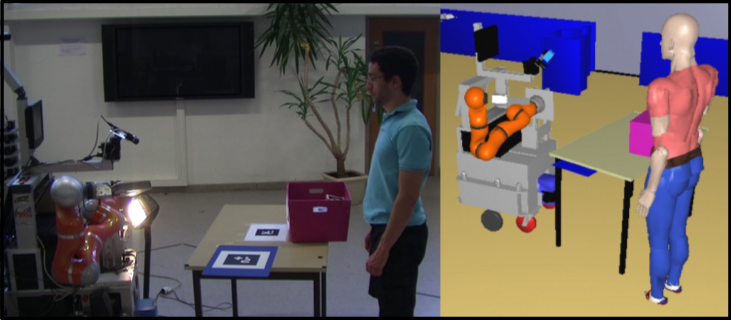
\includegraphics[height=2cm]{manip_run_cam2.png}};
        \node at (t3 -| percept) (cam3) {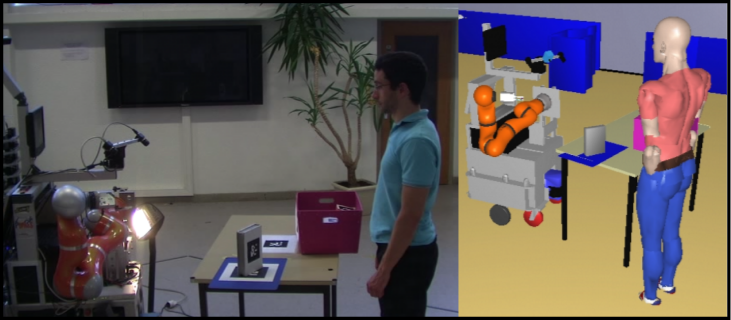
\includegraphics[height=2cm]{manip_run_cam3.png}};
        \node at (t4 -| percept) (cam4) {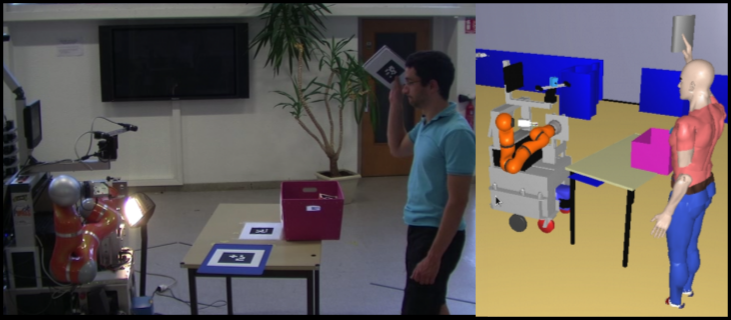
\includegraphics[height=2cm]{manip_run_cam4.png}};
        \node at (t5 -| percept) (cam5) {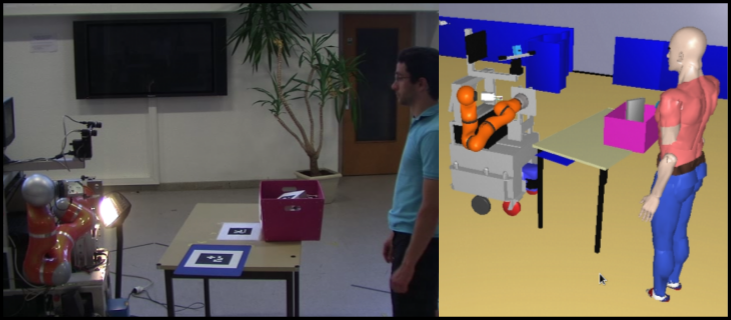
\includegraphics[height=2cm]{manip_run_cam5.png}};

        %%%%%%%%%%%%%%%%%%%%%%%%%%%%%%%%%%%%%%%%%%%%%%%%%%%%%%%%%%%%%%%%%%%%%%%%%%%%%%%%%%%%%%%%%%%%
        %%% KNOWLEDGE
        %%%%%%%%%%%%%%%%%%%%%%%%%%%%%%%%%%%%%%%%%%%%%%%%%%%%%%%%%%%%%%%%%%%%%%%%%%%%%%%%%%%%%%%%%%%%

        \node[fill=white,align=left] at (cam1 -| kbr) (kb1) {\stmt{TAPE isVisible true}\\
                                                        \stmt{TAPE isReachable true}\\
                                                        \stmt{TAPE isOn TABLE}\\
                                                        \stmt{BIN isVisible true}\\
                                                        \stmt{BIN isReachable false}};

        \node[fill=white,align=left] at (cam1 -| kbh) {\stmt{TAPE isVisible true}\\
                                                        \stmt{TAPE isReachable false}\\
                                                        \stmt{TAPE isOn TABLE}\\
                                                        \stmt{BIN isVisible true}\\
                                                        \stmt{BIN isReachable true}};

        \node[fill=white,align=left] at (cam2 -| kbr) (kb2) {\stmt{ROBOT hasInHand TAPE}};


        \node[fill=white,align=left] at (cam3 -| kbr) {\stmt{TAPE isReachable true}\\
                                            \stmt{TAPE isVisible true} \\
                                            \stmt{TAPE isOn TABLE}};

        \node[fill=white,align=left ] at (cam3 -| kbh) (kb3) {\stmt{TAPE isReachable true}\\
                                             \stmt{TAPE isVisible true}};

        \node[fill=white,align=left] at (cam4 -| kbh) (kb4) {\stmt{HUMAN hasInHand TAPE}};

        \node[fill=white,align=left] at (cam5 -| kbr)  {\stmt{TAPE isIn BIN}};
        \node[fill=white,align=left] at (cam5 -| kbh) (kb5) {\stmt{TAPE isIn BIN}};

        %%%%%%%%%%%%%%%% %%%%%%%%%%%%%%%%%%%%%%%%%%%%%%%%%%%%%%%%%%%%%%%%%%%%%%%%%%%%%%%%%%%%%%%%%%%%
        %%% PLANS
        %%%%%%%%%%%%%%%%%%%%%%%%%%%%%%%%%%%%%%%%%%%%%%%%%%%%%%%%%%%%%%%%%%%%%%%%%%%%%%%%%%%%%%%%%%%%

        \node[fill=gray!10!white,below=1 of plan] (incoming) {\bf \Large Incoming goal \\ \it Clean the table!};

        \node[anchor=north, plan, robot] at (cam1.south -| probot) (pr1) {\action{TAKE}{TAPE}{TABLE}};
        \node[anchor=north, plan, robot] at (cam2.south -| probot)  (pr2) {\action{PUTRV}{TAPE}{TABLE}} edge[<-] (pr1);
        \node[anchor=north, plan] at (cam3.south -| phuman) (ph1) {\action{TAKE}{TAPE}{TABLE}} edge[<-] (pr2);
        \node[anchor=north, plan]  at (cam4.south -| phuman) (ph2) {\action{PUT}{TAPE}{BIN}} edge[<-] (ph1);

        \node[fill=gray!10!white,anchor=north] at (cam5.south -| plan) (done) {\bf \Large Goal completed};

        %%%%%%%%%%%%%%%%%%%%%%%%%%%%%%%%%%%%%%%%%%%%%%%%%%%%%%%%%%%%%%%%%%%%%%%%%%%%%%%%%%%%%%%%%%%%
        %%% ACTIONS
        %%%%%%%%%%%%%%%%%%%%%%%%%%%%%%%%%%%%%%%%%%%%%%%%%%%%%%%%%%%%%%%%%%%%%%%%%%%%%%%%%%%%%%%%%%%%

        \node[fill=white] at (pr1 -| arobot) (ep1) {\it evaluate pre-conditions};

        \node[below=0.1 of ep1] (mhp1) {%
            \begin{tikzpicture}
                \node[fill=white] (title) {\bf motion planning};
                \node[below=0.1 of title.south west, label=below:{\tt PICK\_GOTO}] (mapg) {
\includegraphics{MHP_ARM_PICK_GOTO}};
                \node[fill=white,right=of mapg, label=below:{\tt TAKE\_TO\_FREE}] (mattf) {
\includegraphics{MHP_ARM_TAKE_TO_FREE}} edge[<-] (mapg);
            \end{tikzpicture}
        };
        \node[fill=white,below=0.1 of mhp1] (me1) {\bf motion execution};
        \node[fill=white,below=0.1 of me1] (ae1) {\it assess post-conditions};

        %%%%%%%%%%%%%%%%%%%%%%%%%%%%%%%%%%%%%%%%%%%%%%%%%%%%%%%%%%%%%%%%%%%%%%%%%%%%%%%%%%%%%%%%%%%%%
        \node[fill=white] at (pr2 -| arobot) (ep2) {\it evaluate pre-conditions};

        \node[below=0.1 of ep2] (mhp2) {%
            \begin{tikzpicture}
                \node[fill=white] (title) {\bf motion planning};
                \node[fill=white,below=0.1 of title, label=below:{\tt ESCAPE}] (maeo) {
\includegraphics{MHP_ARM_ESCAPE_OBJECT}};
                \node[left=of maeo, label=below:{\tt PLACE\_FROM\_FREE}] (mapff) {
\includegraphics{MHP_ARM_PLACE_FROM_FREE}} edge (maeo);
                \node[fill=white,right=of maeo, label=below:{\tt TO\_FREE}] (maf) {
\includegraphics{MHP_ARM_FREE}} edge[<-] (maeo);
            \end{tikzpicture}
        };
        \node[fill=white,below=0.1 of mhp2] (me2) {\bf motion execution};
        \node[fill=white,below=0.1 of me2] (ae2) {\it assess post-conditions};

        %%%%%%%%%%%%%%%%%%%%%%%%%%%%%%%%%%%%%%%%%%%%%%%%%%%%%%%%%%%%%%%%%%%%%%%%%%%%%%%%%%%%%%%%%%%%%

        \node[anchor=north] at (ph1 -| ahuman) (wait1) {%
            \begin{tikzpicture}
                \node[fill=white] (title) {\it wait for pick\\ {\tt TAPE} \it from {\tt TABLE}};
                \node[below=0.1 of title] {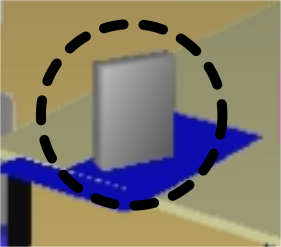
\includegraphics{wait_for_pick}};
            \end{tikzpicture}
        };

        \node[anchor=north] at (ph2 -| ahuman) (wait2) {%
            \begin{tikzpicture}
                \node[fill=white] (title) {\it wait for put\\ {\tt TAPE} \it into {\tt BIN}};
                \node[below=0.1 of title] {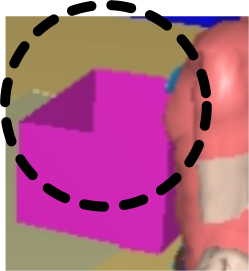
\includegraphics{wait_for_throw}};
            \end{tikzpicture}
        };


        %%%%%%%%%%%%%%%%%%%%%%%%%%%%%%%%%%%%%%%%%%%%%%%%%%%%%%%%%%%%%%%%%%%%%%%%%%%%%%%%%%%%%%%%%%%%
        %%% FLOW
        %%%%%%%%%%%%%%%%%%%%%%%%%%%%%%%%%%%%%%%%%%%%%%%%%%%%%%%%%%%%%%%%%%%%%%%%%%%%%%%%%%%%%%%%%%%%
        \draw[dotted, ->, in=45, out=180] (incoming.west) to (kb1);
        \draw[dotted, ->, bend right] (kb1) to (pr1);
        \draw[dotted, ->, bend left] (pr1) to (ep1);
        \draw[dotted, ->, in=45, out=180] (ae1.west) to (kb2);
        \draw[dotted, ->, bend right] (kb2) to (pr2);
        \draw[dotted, ->, bend left] (pr2) to (ep2);
        \draw[dotted, ->, in=45, out=180] (ae2.west) to (kb3);
        \draw[dotted, ->, bend right] (kb3) to (ph1);
        \draw[dotted, ->, bend left] (ph1) to (wait1);
        \draw[dotted, ->, in=-20, out=180] (wait1.west) to (kb4.east);
        \draw[dotted, ->, bend right] (kb4) to (ph2);
        \draw[dotted, ->, bend left] (ph2) to (wait2);
        \draw[dotted, ->, in=20, out=180] (wait2.west) to (kb5);
        \draw[dotted, ->, bend left] (kb5.east) to (done.north);


 \end{tikzpicture}
 }

 \caption {Timeline of the \emph{Cleaning the table} study, presented here in a simplified
 version: a single object, {\tt TAPE}, must be removed from the table and
 dropped in the bin {\tt BIN}. The light arrows sketch the global execution
 flow.}

  \label{fig|cleantable-timeline}
\end{figure*}


%The plan produced in that case by HATP is straightforward and shown in the
%third row. It consists of four successive actions involving the robot and the
%human. Robot grasps the tape and then places it on the table at a position
%where it is visible and reachable for the human. The human is then asked to pick
%the tape and throw it in the trashbin.

%%%%%%%%%%%%%%%%%%%%%%%%%%%%%%%%%%%%%%%%%%%%%%%%%%%%%%%%%%%%%%%%%%%%%%%%%%%%%%%%
%%%%%%%%%%%%%%%%%%%%%%%%%%%%%%%%%%%%%%%%%%%%%%%%%%%%%%%%%%%%%%%%%%%%%%%%%%%%%%%%
%%%%%%%%%%%%%%%%%%%%%%%%%%%%%%%%%%%%%%%%%%%%%%%%%%%%%%%%%%%%%%%%%%%%%%%%%%%%%%%%

\section{Discussion: When Artificial Intelligence Enables Human-Robot
Interaction}
\label{sect|discussion}

The previous sections provide a perspective on a complete deliberative
architecture for social robots, including an implementation supported
``real-world'' experimental deployments. This section synthesises next what we
see as the main challenges that human-robot interaction brings to Artificial
Intelligence.  We discuss first how embodied cognition is a very real challenge
in human-robot interaction; we rephrase then the requirements of joint actions
in terms of five questions; we discuss the importance of building and
maintaining a multi-level model of the human; and we finally reflect on the
importance of explicit knowledge management in robotic architectures that deal
with human-level semantics and state in that respect the current limits of our
logic framework.

\subsection{Embodied Cognition}

Robotics is traditionally regarded as the prototypical instance of
\emph{embodied} artificial intelligence, and this dimension is especially
prevalent in human-robot interaction, where agents have to share and
collaborate in a joint physical environment.  This leads to a tight coupling
between the symbolic and the geometric realms: while AI at its origins was
mostly concerned with symbolic models, it has been since recognised that not
only the mind is not a purely abstract system, disconnected from the physical
world, but even more, cognition fundamentally relies on its relation to the
physical world (so-called \emph{embodied cognition}). Varela~\cite{Varela1992}
is one of the main discoverers of these mechanisms, and coined the concept of
\emph{enactivism} as the theoretical framework that studies the links between
cognition, embodiment and actions.  This has since been thoroughly studied in
robotics and artificial intelligence (Pfeifer and
Bongard~\cite{pfeifer2007body} is one of the reference).

The challenge of symbol grounding is also tightly linked to this issue. It
corresponds to the identification or creation, and then, maintenance of a link
between the symbol (the syntactic form of knowledge that the computer
manipulates) and its semantics (its meaning, anchored in the world). The
relation between the symbol, the referent of the symbol, and mediating minds
is classically referred as the \emph{semantic triangle} and has been
extensively studied in linguistics. The issue of grounding is well known in
cognitive science and is summarised by Harnad~\cite{Harnad1990} by this
question: ``how the semantic interpretation of a formal symbol system can be
made intrinsic to the system?''. This issue has a major practical importance in
robotic: for a robot to be both endowed with a symbolic representational and
reasoning system, and able to \emph{act} in the physical world, it must ground
its knowledge.

As we have seen, grounding is implemented at different levels in our
architecture. The main source of grounded symbolic knowledge is the situation
assessment module, {\sc Spark}. It builds symbolic facts from spatial reasoning,
and also relies on (limited) temporal reasoning to track the world state and
build explanations to interpret unexpected perceptions (like an object that
suddendly disappears). Because {\sc Spark} also tracks humans, which enables
perspective-aware spatial reasoning, it can produce as well grounded symbolic
knowledge for the agents it interacts with. This is a typical \emph{embodied}
cognitive skill.

Grounding also occurs during verbal and non-verbal communication. The {\sc
Dialogs} module grounds new concepts introduced by the speaker by asking
questions until it can attach the new concept to concepts already present in the
knowledge pool (if one asks the robot ``bring me a margarita'', the robot may
initially asks ``what is a margarita?''. The user would answer ``a cocktail''
and the robot would continue the grounding -- ``what is a cocktail?'' -- until
it anchors the new concept to ones it already knows). Embodied interactions
(like gestures) are also taken into account at this level: we have presented how
pointing, for instance, is used by the robot to ground \emph{``this''} or
\emph{``that''} to the pointed artifact.

Note that, because only objects marked with 2D fiducial markers are currently
recognised (typically, about ten of them are simultaneously used in a given
experiment), our grounding mechanisms have only been exercised in small-sized
closed world. This simplifies the task, and we can not claim that our approach
provides a generic grounding capability. Beyond the perception of geometric
entities, context, cultural background, ``naive physics'' knowledge, emotional
state of the human are some of the numerous other determinants that need to be
accounted for when grounding human-robot interaction.

\subsection{The W-questions of Joint Action}

Our context, where a robot has to achieve a task together with
humans, raises issues to be tackled by the robots' decisional components, and
that we can summarise as ``W-questions'': \emph{What}, \emph{Who}, \emph{When},
\emph{Where} and \emph{How}?

\emph{What to do next}, at different levels of abstractions and while taking
into account not only the current state but also the long term goals, is the
basic question for an intelligent robot. It is made more complex here by having
to deal with the partially observable physical and mental state of the human
partner, and by the extended set of possible actions.

\emph{Who should act now} is of key importance and also needs to be
decided upon by the robot. It is sometimes expected as an intelligent behaviour
for the robot to wait and let its human partner act instead. Correct management
of \emph{turn-taking} leads to various decisional challenges.

\emph{When to perform a given action} is enriched here by the human context
since it has to take into account the human, his/her needs, his/her rhythms and
pace, and his/her mental state. While performing its share of the task, the
robot has to produce signals directed towards the human and to respond to
signals produced back at the proper pace.

\emph{Where to perform an action} plays an important role as well: the choice is
not trivial and might need elaborated decision. The robot is expected to take
into account effort sharing, visibility of its action by the human, disturbance
or discomfort induced by its action.

\emph{How to perform an action}, finally, needs to be reflected upon by the
robot: several options to perform an action or to achieve a goal are often
available, and selecting one is a non-trivial decision problem. Cost-based
planners are one possible approach: they search for plans that satisfy an
acceptable cost in terms of \emph{acceptability} or \emph{legibility}, for
instance.

These five questions should not be considered independently from each others and
often require, on the contrary, to be dealt with in a single decision step. The
human-aware task and motion planners which we have built, are instances of
systems which have been designed to deal with such intricate decision issues.

\fixme{Rachid: the reviewer 2 asks for a better connection between these general
questions and the specific approaches that we take}

\subsection{Putting the Humans into Equations}

The correlate of these five \emph{W-questions} is the issue the \emph{human
models}: taking appropriate decisions with and in presence of humans requires
appropriate models of the human: what the human \emph{can do}, \emph{would like
to do}, \emph{knows}, \emph{could infer}, etc.

While the task of describing all the (dynamic) human models that are useful to
robots is immense (if doable at all), we claim that it is possible to devise and
use such models in limited, but still interesting and useful, contexts such as
collaborative human-robot objects manipulation, fetch-and-carry and associated
activities in home or work environments.

In our architecture, perspective taking, for instance, is tightly connected to
the symbolic knowledge models, and since our knowledge base allows for storage
of one knowledge model per agent, we have been able to endow the robot with a
simple theory of mind (as explained in section~\ref{sect|tom}): we explicitly
model what the robot knows about its partners in a symbolic way. This knowledge
is then re-used in different places, to correctly interpret what the human says,
or to plan tasks that are actually doable for the human.

The cognitive model that the robot builds for the agents it interacts with
remains today simple and mostly focused on geometric features and affordances
(\emph{who sees what? what are our relative positions? what is reachable to
whom?}). Extending this knowledge with more subtle perceptions (emotional
state for instance) remains to be explored beyond simple examples like the
processing of explicit verbal statements like ``I'm tired!''
(Section~\ref{sect:desires}).

Motion and action execution also requires human models, and the one we use
embeds human preferences and physical constraints that need to be accounted for
when synthesizing robot motion or producing robot plans. This includes
proxemics (human-robot distance) and associated issues (visibility) but also
legibility and acceptability criteria expressed in terms of \emph{social rules}
that the produced plans should satisfy.

%
%\paragraph{Joint actions with humans}\label{sec:soa}
%\fxfatal{too many citation -> synthesis needed!}
%
%The human presence brings new requirements for robot's abilities both
%at the functional and at the deliberative levels~\cite{Klein2004}. The
%topics involve motion~\cite{Kulic2007,Berg2004,Madhava2006},
%navigation~\cite{Althaus2004,Sisbot2007}, manipulation~\cite{Kemp2007}
%in presence of humans as well as perception of human
%activities~\cite{Breazeal2001,Burger2008}. Also, when
%interacting with humans, robots need to incorporate communication and
%collaboration abilities. Several theories dealing with
%collaboration~\cite{Cohen1991,Grosz1996,Clark1996} emphasise that
%collaborative tasks have specific requirements compared to individual
%ones, \eg, since the robot and the person share a common goal, they
%have to agree on the manner to realise it, they must show their
%commitment to the goal during execution, etc. Several robotic systems
%have already been built based on these
%theories~\cite{Rich1997,Sidner2005,Breazeal2003} and they
%all have shown benefits of this approach. They have also shown how
%difficult it is to manage turn-taking between communication partners
%and to interleave task realization and communication in a generic
%way. Finally, today only few
%systems~\cite{Fong2006,Breazeal2003,Sisbot2008} take humans into
%account at all levels.


\subsection{Explicit Knowledge for Social Robotics}
\label{krs-discussion}

As thoroughly presented in this article, we have built the decisional
capabilities of our robots around this idea of explicit knowledge manipulation.
We finally briefly comment on this design choice and the limitations of our
approach.

\subsubsection{Explicit Knowledge in our Architecture}

The components that we have presented so far build a \emph{knowledge-oriented}
architecture: knowledge is explicitly stored in one central and consistent
repository of facts, accessible for all modules. It relies on a strict formalism
(OWL statements), with a well defined vocabulary (stated in the common-sense
ontology). These first two points lead to a loosely-coupled architecture
where modules can be removed or replaced easily by other ones as long as they
share the same semantics: modules are defined by the knowledge they produce or
consume.

Also, we adopt a symbolic, hybrid (reactive and planning-based), event-driven
approach to robot control. By managing events at the same level as the reasoner,
we take full advantage of the inference abilities of {\sc Oro} to trigger events
whose \texttt{true} conditions can be (possibly indirectly) inferred using
human-level semantics.

And finally, this architecture allows for the combination of different
knowledge sources in a uniform model, bringing mutual
benefits to components. For instance, the dialogue processing module can
run without any situation assessment, but its disambiguation routines
can transparently benefit from it when available (since richer symbolic
descriptions of objects are then available).

Those characteristics are not novel \emph{per se}. We want however underline the
shift of focus brought by this approach during the design and integration phases
of robots: components of our deliberative layer are defined and bound together
by the knowledge they produce and consume. Human-robot interaction, because it
supposes operations at \emph{human-level} and in environments with complex
semantics, acts here as a motivational force.


\subsubsection{Limits of Disambiguation at Semantic Level}

Interaction with humans implies the ability to deal with semantics: semantics of
verbal interaction, semantics of gestures, etc.  As a consequence, it also
implies to deal with semantic disambiguation.

We have studied a prototypical example of semantic disambiguation in
\cite{Ros2010b} with the children's ``spygame'': two players are facing
each other with a set of random objects in-between, one player mentally choose
one object, and the other player has to guess the object by asking closed
questions like \emph{Is your object small or large?} Based on the knowledge it
has acquired, the robot is able to minimise the number of questions required to
find the object.

When playing this kind of game, however, the issue arises that the robot has no
way to select which knowledge about the object is relevant in the interaction
context. For instance, the knowledge base may store facts like \stmt{obj1 type
ActiveConcept} (which internally means that this concept was mentioned in a
discussion in the last few seconds): this information is not a relevant
property of \concept{obj1} when trying to disambiguate concepts with humans.
This distinction between \emph{internal knowledge} (meaningful to
the system only) and \emph{common knowledge} (whose meaning is understood by
all the interactors) has not been properly dealt with in our architecture.

Besides, even knowledge that belongs to the \emph{common knowledge} may not be
appropriate in a given interaction context. For instance, the system may
compute that at a given instant the human is looking at the object: \stmt{human
looksAt obj1}. This property makes sense to both parties, but in the context of
the \emph{spygame}, we would like to mainly use immanent properties, not
volatile like a gaze. More research is required to identify relevant
interaction contexts and knowledge classes attached to them.

\section{Conclusion}
\label{sect|conclusion}

\subsection{A Deliberative Architecture for Social Robots}

We have presented in this paper a large deliberative architecture designed for
social robots. While most of its sub-components have been independently
presented in other publications, we offer here for the first time a perspective
on the overall integration of these components into a coherent and consistent
system for social human-robot interaction. We have first exposed our underlying
knowledge model based on Description Logics~\cite{Lemaignan2010} and some of the
resulting reasoning capabilities pertaining to disambiguation~\cite{Ros2010b}
and mental modelling~\cite{warnier2012when} that are shown to effectively
scaffold interaction using human-level semantics and cognitive skills. We have
then presented our approach to symbol grounding, build on an amodal situation
assessment environment~\cite{Sisbot2011} that supports perspective
taking~\cite{Marin2008,Ros2010}. We
combine it further with an advanced natural
language processor~\cite{Lemaignan2011a} to provide complete multi-modal interactive
communication.  The paper also covers our symbolic social task
planner~\cite{Alili2008, Alili2009, Lallement2014}: it generates predictive
plans of the human actions that enable the system to plan for joint human-robot
tasks. It can also make use of social heuristics to optimize plans for social
acceptability. We briefly mention our human-aware motion and manipulation
planner~\cite{Sisbot2008,Mainprice2011,Pandey2011}, and finally present two
execution controller, the PRS-based {\sc Shary}~\cite{clodic2008shary,fiore2014} and the
event-driven {\sc pyRobots}~\cite{lemaignan2015pyrobots}.

The integration of these components in a consistent, working and observable
system is supported by the design of our software interfaces: most of the
datastreams exchanged by our components uses high-level semantics in the form of
first-order logic statements. The two reported support studies further evidence
how our use of explicit, high-level semantics provide a low-impedance,
human-level mean of building a complex deliberative
architecture for socially interactive robots~\cite{Lemaignan2013}.


\fixme{Rachid -- TDB: what are the other 'deliberative architecture for socially interactive
robots' and where/how ours is better?}


While several contributions in the literature provide insights and contributions 
on one aspect or another, we are not aware of a fully implemented architecture that effectively
combines in a coherent manner all the points mentioned above.
We do not claim that this represents the only architecture that can be designed
to address such problems, nor that our approach fully addresses each and every
of these issues. Our point here is that it is a fully implemented architecture that allowed us to
identify, refine and combine a number of key cognitive abilities that we believe are necessary. Indeed, 
we show here below that it provided us a mean to develop and explore a number of key features for HRI 
in terms of models and algorithms and their articulation in an integrated decisional system for a 
cognitive and interactive robot.



\fixme{Discussion on deliberative architectures != cognitive architecture}: a \emph{cognitive
architecture} is usually understood as an artificial yet principled model of (human)
cognition, while we propose a practical approach to consistently combine a large
set of independent cognitive processes by bridging them through high-level semantics.

\subsection{The Next Steps}

%We have presented in this article a decisional framework for human-robot
%interactive task achievement that is aimed to allow the robot not only to
%accomplish its tasks but also to produce behaviours that support its engagement
%vis-a-vis its human partner and to interpret human behaviours and intentions.
%Together and in coherence with this framework, we have developed and
%experimented various task planners and interaction schemes that allow the robot
%to select and perform its tasks while taking into account explicitly the human
%abilities as well as the constraints imposed by the presence of humans, their
%needs and preferences. 

The design choices and the results presented here are still preliminary.
While the general scheme we propose might be difficult to implement in
a general sense, we believe that it is a reasonable challenge to
implement it in the case of a personal robot assistant essentially
devoted interactive manipulation
tasks and associated activities.

One direction that we would like to further investigate is how to account for
situations where divergent beliefs appear between the human and the robot.
Preliminary results have been published in~\cite{warnier2012when}.

There is also extensive work to be done in order to refine the notion of ``good
shared plan'' and ``good/acceptable robot behaviour'' in this context. There are
obviously large avenues for learning and adaptation in this context.

Another direction to head to deals with \emph{contexts representation}.
Contexts are currently often limited to the current spatial and temporal
situation. Some models offer the possibility to jump in the past or to switch to
another agent's perspective, but in current approaches, selecting a context
always basically consists in retrieving a set of beliefs corresponding to a
situation, and temporarily replacing the current beliefs by those other ones.
This misses the fact that at a given moment, not one but many contexts co-exist
at different scales. We do not want to retrieve one monolithic set of beliefs,
but instead carefully craft a context from several \emph{atomic} contexts.
Techniques for representation of overlapping pools of knowledge largely remain
to be developed, as well as efficient algorithms to retrieve (or discard) such
context-related pools of knowledge. This is a challenge not only for robotics,
but more generally for artificial intelligence.  The ability to explicitly
manage contexts and context switches would endow the robot with a cognitive
capability similar to what is known as \emph{context-dependent memory} in
cognitive psychology. This is also related to Tulving's \emph{autonoetic
consciousness}~\cite{Tulving1985a}: the ability to reflect upon its own past or
future experiences.  Much remain to be done to this regard, starting with a
formal analysis of what are the relevant contexts for our robots.

Human-Robot Interaction is and is going to remain a challenging field for
Artificial Intelligence. We hope that this contribution helps with clarifying
some of these challenges.

\section*{Acknowledgements}

Building such a robotic architecture is the work of many hands, and we would
like to acknowledge here the worthwhile contributions of Samir Alili, Raquel Ros
Espinoza, Mamoun Gharbi, Julien Guitton, Matthieu Herrb, Jim Mainprice and Amit
Kumar Pandey.

This work has been partially supported by EU FP7 ``SAPHARI'' (grant ICT-287513),
and the EU H2020 Marie Sklodowska-Curie Actions project DoRoThy (grant 657227).



\bibliographystyle{elsarticle-num}
%\bibliographystyle{abbrv}
\bibliography{laas_hri,other_citations}



\end{document}
